\documentclass[debug]{phd}

\begin{document}
%%
\ensurepagenumbering{arabic}
%%	
	%
	\chapter{Differential Geometry Preliminaries}
	\label{chap1}
		%
		In this chapter we introduce the needed mathematical notions for this thesis. 
		In particular, we collect some definitions about $G$-structures, holonomy and torsion, in order to generalise them to the generalised analogous in the next chapter.
		These concepts are the mathematical way to encode the topological and differential conditions on the internal manifold coming from supersymmetry in string compactifications. 
		
		We will see in the following how precisely relate the existence and the integrability of $G$-structures to the supersymmetry of the compactified theory.
		
		\section{Introduction and Motivations}
			%
				We are mainly interested in compactifications and dimensional reductions of 10 or 11-dimensional supergravity preserving a certain fraction of the original supersymmetry. We take the ansatz for spacetime solutions to be in the form
					%
						\begin{equation}\label{spacetimeans}
							M = X \times M_{d}\, ,
						\end{equation}
where $X$ is a Lorentzian (\emph{external}) spacetime and $M_{d}$ is a Riemannian manifold, often called \emph{internal} space.
In order to have supersymmetry in the lower dimensional theory, the internal manifold must support spinors, namely they must be \emph{spin manifolds}.
The supersymmetry parameters in $D=10$ or $D=11$ dimensional are generically indicated by $\epsilon$ and transform in the fundamental representation of $\mathrm{Spin}(D-1,1)$.
The number of supersymmetries the lower dimensional theory is given by the decomposition ansatz for the higher dimensional supersymmetry parameters
				\begin{equation*}
				 \epsilon = \sum_{k=1}^\mathcal{N} \varepsilon^k \otimes \eta^k\, .
				\end{equation*}

				The $\varepsilon^k$ are the lower dimensional supersymmetry parameters, \emph{i.e.} $\mathrm{Spin}(D-d-1,1)$ spinors, while $\eta^k$ are commuting $\mathrm{Spin}(d)$ spinors.
				The number $\mathcal{N}$ of linearly independent spinors $\varepsilon^k$ is the number of supersymmetries of the lower dimensional theory.
				
In order to make sense of the supersymmetry in lower dimension, we assume that the internal spinors $\eta^k$ are globally defined. 
As we will see in the next section, this is a non-trivial topological condition, that imposes the reduction of the structure group of the internal manifold.
				%
			%
		\section{\texorpdfstring{$G$-structures}{G-structures}}
			\label{gstruc}
			%
					Let $M$ be a manifold of real dimension $d$ and $TM$ is tangent bundle. 
					At any point $p \in M$ we can introduce a local basis, and write a generic vector $v$ as
						%
							\begin{equation}
								v = v^a_{(\alpha)} e_a^{(\alpha)}\, .
							\end{equation}
						%
					Its coordinates on the overlap of two patches, $U_\alpha \cap U_\beta$, are related by a local change of coordinates,
						%
							\begin{align}
								v^a_{(\alpha)} = M_{\alpha\beta\phantom{a} b}^{\phantom{\alpha \beta}a}\ v^b_{(\beta)}\, ,
							\end{align}
						%
					where the transformation $M_{\alpha\beta}$ is in $\GL(d, \mathbb{R})$.
					Since the construction depend on the point $p \in M$, the matrices $M_{\alpha\beta}$ can be seen as maps from the manifold to the group $\GL(d, \mathbb{R})$,
						%
							\begin{equation*}
								\begin{tikzcd}[row sep=.3mm]
									M_{\alpha \beta} :\!\!\!\!\!\!\!\!\!\!\!\!\!\!\!\!\! & M \arrow{r} & \GL(d, \mathbb{R}) \\
 									& p \arrow[mapsto]{r} & M_{\alpha \beta}(p)
								\end{tikzcd}
							\end{equation*}
						%
					and are called \emph{transition functions}. 
					They contain all the information about the non-trivial topology of the tangent bundle.
					The following cocycle condition is required on the triple overlap for consistency,
						%
							\begin{equation}
								M_{\alpha\beta} M_{\beta\gamma} = M_{\alpha\gamma}\, ,
							\end{equation}
						%
					and in addition,
						%
							\begin{equation}
								M_{\alpha\beta}M_{\beta\alpha} = 1\, .
							\end{equation}
						%
					Note that the last two equations are the closure and the existence of the identity axioms in a group. 
					The group $\GL(d, \mathbb{R})$ of transition functions\footnote{%
					One can define the transition functions also as the action of the group on the fibre, in order to change local frame.
						This is also mentioned above and it is related to the interpretation of active/passive transformations.%
						} %
					is called the \emph{structure group} of the tangent bundle.
						%
													%
						
						
						We call \emph{Frame bundle} on $M$ the principal bundle whose fibres at any point $p \in M$ are all ordered basis -- \emph{i.e.} the frames -- of the tangent space $T_p M$, 
					%
						\begin{equation}\label{framebund}
							F = \bigsqcup_{p \in M} F_p\, ,
						\end{equation}
					%
				where,
					%
						\begin{equation}
							F_p := \left\{ (p, \{ e_a \}) \mid p \in M \right\}\, .
						\end{equation}
					%
				Generically, one can identify the fibre with $\GL(d,\mathbb{R})$.
				The group $\GL(d,\mathbb{R})$ acts freely and transitively on each fibre on the right - \emph{i.e.} $F_p$ is a principal homogeneous space for $\GL(d,\mathbb{R})$ -- to give another frame on the fibre. 
				From this point of view we can see the action of the group $\GL(d,\mathbb{R})$ as the way of changing frames keeping the point $p \in M$ fixed, so the change of frame is a transformation on the fibre only, see~\cref{gactfibre}.
				
				The set $\{e^{(\alpha)}_a\}$ defines in general a local frame on the manifold $M$ over the patch $U_{\alpha}$, namely a set of $d$ vector fields spanning $T_p M$. 
				Generally, it might not be possible to define it over the whole manifold, as it might not be possible to cover the manifold with a single chart.
				The particular case where a \emph{global frame} is defined is when the manifold is \emph{parallelisable}. 
				A noteworthy example of parallelisable manifolds are Lie groups. 
				This notion will be important for this work and we will discuss it -- and its generalisation in Generalised Geometry -- in detail in the next chapter.
				
				For simplicity we will present the various definitions using the tangent bundle, however, these and the related properties hold also for more general bundles $E$ on $M$, with a generic vector space $V$ as fibre, with a group $G$ acting on $V$.
						
						\begin{figure}[h]
							\centering
								\scalebox{1.5}{\documentclass{standalone}

\usepackage{amsmath, amssymb, amsfonts, amscd, amsthm, bigints, units}
%!TEX encoding = UTF-8 Unicode
\usepackage{tikz}
\usepackage{tikz-cd}
\usepackage{tikz3dcs-pp}
\usepackage{pgfplots}
\usepackage{xcolor, eecolors}
\usepackage{math, lrmath}

\usepackage{pgfplots}
\usepgfplotslibrary{patchplots}
\pgfplotsset{compat=1.15}

\usetikzlibrary{calc, intersections}

\usetikzlibrary{decorations.pathmorphing,calc,shapes,positioning,fit,arrows,fadings,decorations.pathreplacing,decorations.pathmorphing,intersections,patterns, trees}
\usetikzlibrary{decorations.markings}

\usepackage{marvosym}

%%%%%%%%My Tikz definitions%%%%%%%%%%%%%%%%%
\tikzset{->-/.style={decoration={
  markings,
  mark=at position #1 with {\arrow{latex}}},postaction={decorate}}}
  %
\tikzset{
    %Define standard arrow tip
    >=stealth',
    %Define style for boxes
    punkt/.style={
           rectangle,
           rounded corners,
           draw=black, very thick,
           text width=7.5em,
           minimum height=2em,
           text centered},
    % Define arrow style
    pil/.style={
           ->,
           thick,
           shorten <=2pt,
           shorten >=2pt,}
}
%%%
%%3d drawings %%%
\newcommand\pgfmathsinandcos[3]{%
  \pgfmathsetmacro#1{sin(#3)}%
  \pgfmathsetmacro#2{cos(#3)}%
}
\newcommand\LongitudePlane[3][current plane]{%
  \pgfmathsinandcos\sinEl\cosEl{#2} % elevation
  \pgfmathsinandcos\sint\cost{#3} % azimuth
  \tikzset{#1/.style={cm={\cost,\sint*\sinEl,0,\cosEl,(0,0)}}}
}
\newcommand\LatitudePlane[3][current plane]{%
  \pgfmathsinandcos\sinEl\cosEl{#2} % elevation
  \pgfmathsinandcos\sint\cost{#3} % latitude
  \pgfmathsetmacro\yshift{\cosEl*\sint}
  \tikzset{#1/.style={cm={\cost,0,0,\cost*\sinEl,(0,\yshift)}}} %
}
\newcommand\DrawLongitudeCircle[2][1]{
  \LongitudePlane{\angEl}{#2}
  \tikzset{current plane/.prefix style={scale=#1}}
   % angle of "visibility"
  \pgfmathsetmacro\angVis{atan(sin(#2)*cos(\angEl)/sin(\angEl))} %
  \draw[current plane] (\angVis:1) arc (\angVis:\angVis+180:1);
  \draw[current plane,dashed] (\angVis-180:1) arc (\angVis-180:\angVis:1);
}
\newcommand\DrawLatitudeCircle[2][1]{
  \LatitudePlane{\angEl}{#2}
  \tikzset{current plane/.prefix style={scale=#1}}
  \pgfmathsetmacro\sinVis{sin(#2)/cos(#2)*sin(\angEl)/cos(\angEl)}
  % angle of "visibility"
  \pgfmathsetmacro\angVis{asin(min(1,max(\sinVis,-1)))}
  \draw[current plane] (\angVis:1) arc (\angVis:-\angVis-180:1);
  \draw[current plane,dashed] (180-\angVis:1) arc (180-\angVis:\angVis:1);
}
%%%%


\tikzset{every node/.style={font=\tiny}}

\begin{document}
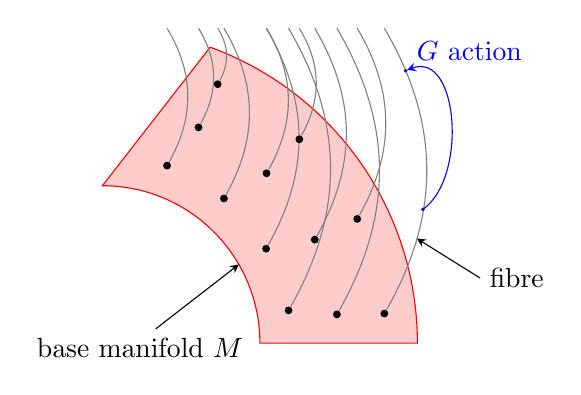
\begin{tikzpicture}[>=stealth]
%\draw[color=red](2,0)--(4,0)node[midway,below]{\textcolor{black}{fibre bundle}}arc(0:70:4)--(90:2)arc(90:0:2)--cycle;
\draw[color=red](2,0)--(4,0)arc(0:70:4)--(90:2)arc(90:0:2)--cycle;
\fill[fill = red, opacity = .2] (2,0)--(4,0)arc(0:70:4)--(90:2)arc(90:0:2)--cycle;

\draw[->] (15:0.7)node[below,xshift=-2mm]{base manifold $M$}--(30:2);

\begin{scope}[bend right]
\foreach \i[count=\x] in {10,30,50,70}
{\node(a\x)[circle,fill,inner sep=1pt]at (\i:2.4){};
\draw[color= gray](a\x)to(a\x|-0,4);}

\foreach \i[count=\x] in {7,26,46,66}
{\node(b\x)[circle,fill,inner sep=1pt]at (\i:3){};
\draw[color= gray](b\x)to(b\x|-0,4);}

\foreach \i[count=\x] in {6,26,46,66}
{\node(c\x)[circle,fill,inner sep=1pt]at (\i:3.6){};
\draw[color= gray](c\x)to(c\x|-0,4);}

\path(c1)to coordinate[near start](d)(c1|-0,4);
\end{scope}
\draw[<-](d)--+(0.8,-0.5)node[right]{fibre};
\draw[->, color=blue](4.07,1.7) to [out=35, in= 20] +(-.2,1.77)node[above right]{$G$ action};
\node(e)[circle, fill, color=blue, inner sep=.5pt] at (4.07,1.7){};
\node(f)[circle, fill, color=blue, inner sep=.5pt] at (3.85,3.46){};

\end{tikzpicture}
\end{document}
}
								\caption{The action of the structure group on the frame bundle is an action on the fibre only, leaving the point $p \in M$ untouched.}
								\label{gactfibre}
							\end{figure}
						
					An alternative definition of the structure group is the group of the transition functions of the frame bundle $F$ in~\eqref{framebund}.
					Since a vector field $v$ is invariant across patches, we have that the frames transform with the inverse transformation with respect to the vector components,
						%
							\begin{align}
								& & & & & & e_a^{(\alpha)} = M_{\alpha\beta\, a }^{\phantom{\alpha \beta a} b }\ e_b^{(\beta)}\, ,& & \mbox{on}\quad U_\alpha \cap U_\beta \, .& & & &
							\end{align}
						%
					One can notice that given a reference frame, \emph{e.g.} the coordinate one $e_a \equiv \partial_a$, one can obtain a generic local frame via,
						%
							\begin{equation}
								e^{\alpha}_a = e^{\alpha\phantom{a}b}_a \partial_b\, ,
							\end{equation}
						%
					where $e^{\alpha\phantom{a}b}_a$ can be considered as $\GL(d,\mathbb{R})$ elements, giving us the right to identify the fibre of the frame bundle with the $\GL(d, \mathbb{R})$ group.
					
						%
							\begin{figure}[h]
							\centering
								%
									\scalebox{1}{\documentclass[border=5mm,tikz]{standalone}

\usepackage{amsmath, amssymb, amsfonts, amscd, amsthm, bigints, units}
%!TEX encoding = UTF-8 Unicode
\usepackage{tikz}
\usepackage{tikz-cd}
\usepackage{tikz3dcs-pp}
\usepackage{pgfplots}
\usepackage{xcolor, eecolors}
\usepackage{math, lrmath}

\usepackage{pgfplots}
\usepgfplotslibrary{patchplots}
\pgfplotsset{compat=1.15}

\usetikzlibrary{calc, intersections}

\usetikzlibrary{decorations.pathmorphing,calc,shapes,positioning,fit,arrows,fadings,decorations.pathreplacing,decorations.pathmorphing,intersections,patterns, trees}
\usetikzlibrary{decorations.markings}

\usepackage{marvosym}

%%%%%%%%My Tikz definitions%%%%%%%%%%%%%%%%%
\tikzset{->-/.style={decoration={
  markings,
  mark=at position #1 with {\arrow{latex}}},postaction={decorate}}}
  %
\tikzset{
    %Define standard arrow tip
    >=stealth',
    %Define style for boxes
    punkt/.style={
           rectangle,
           rounded corners,
           draw=black, very thick,
           text width=7.5em,
           minimum height=2em,
           text centered},
    % Define arrow style
    pil/.style={
           ->,
           thick,
           shorten <=2pt,
           shorten >=2pt,}
}
%%%
%%3d drawings %%%
\newcommand\pgfmathsinandcos[3]{%
  \pgfmathsetmacro#1{sin(#3)}%
  \pgfmathsetmacro#2{cos(#3)}%
}
\newcommand\LongitudePlane[3][current plane]{%
  \pgfmathsinandcos\sinEl\cosEl{#2} % elevation
  \pgfmathsinandcos\sint\cost{#3} % azimuth
  \tikzset{#1/.style={cm={\cost,\sint*\sinEl,0,\cosEl,(0,0)}}}
}
\newcommand\LatitudePlane[3][current plane]{%
  \pgfmathsinandcos\sinEl\cosEl{#2} % elevation
  \pgfmathsinandcos\sint\cost{#3} % latitude
  \pgfmathsetmacro\yshift{\cosEl*\sint}
  \tikzset{#1/.style={cm={\cost,0,0,\cost*\sinEl,(0,\yshift)}}} %
}
\newcommand\DrawLongitudeCircle[2][1]{
  \LongitudePlane{\angEl}{#2}
  \tikzset{current plane/.prefix style={scale=#1}}
   % angle of "visibility"
  \pgfmathsetmacro\angVis{atan(sin(#2)*cos(\angEl)/sin(\angEl))} %
  \draw[current plane] (\angVis:1) arc (\angVis:\angVis+180:1);
  \draw[current plane,dashed] (\angVis-180:1) arc (\angVis-180:\angVis:1);
}
\newcommand\DrawLatitudeCircle[2][1]{
  \LatitudePlane{\angEl}{#2}
  \tikzset{current plane/.prefix style={scale=#1}}
  \pgfmathsetmacro\sinVis{sin(#2)/cos(#2)*sin(\angEl)/cos(\angEl)}
  % angle of "visibility"
  \pgfmathsetmacro\angVis{asin(min(1,max(\sinVis,-1)))}
  \draw[current plane] (\angVis:1) arc (\angVis:-\angVis-180:1);
  \draw[current plane,dashed] (180-\angVis:1) arc (180-\angVis:\angVis:1);
}
%%%%


\begin{document}

\begin{tikzpicture}

%    % Functions i
%    \path[->] (0.8, 0) edge [bend right] node[left, xshift=-2mm] {$\phi_i$} (-1, -2.9);
%    \draw[white,fill=white] (0.06,-0.57) circle (.15cm);
%    \path[->] (-0.7, -3.05) edge [bend right] node [right, yshift=-3mm] {$\phi^{-1}_i$} (1.093, -0.11);
%    \draw[white, fill=white] (0.95,-1.2) circle (.15cm);
%
%    % Functions j
%    \path[->] (5.8, -2.8) edge [bend left] node[midway, xshift=-5mm, yshift=-3mm] {$\phi^{-1}_j$} (3.8, -0.35);
%    \draw[white, fill=white] (4,-1.1) circle (.15cm);
%    \path[->] (4.2, 0) edge [bend left] node[right, xshift=2mm] {$\phi_j$} (6.2, -2.8);
%    \draw[white, fill=white] (4.54,-0.12) circle (.15cm);

    	% Manifold
	\draw[smooth cycle, tension=0.4, fill=white, pattern color=brown, pattern=north west lines, opacity=0.5] plot coordinates{(2,2) (-0.5,0) (3,-2) (5,1)} node at (0,0) {$M$};

    	% Help lines
    	%\draw[help lines] (-3,-6) grid (8,6);

    	% Subsets
    	\draw[smooth cycle, pattern color=orange, pattern=crosshatch dots] 
        		plot coordinates {(1,0) (1.5, 1.2) (2.5,1.3) (2.6, 0.4)} 
        		node [label={[label distance=-0.3cm, xshift=-2cm, fill=white]:$U_\alpha$}] {};
    	\draw[smooth cycle, pattern color=blue, pattern=crosshatch dots] 
        		plot coordinates {(4, 0) (3.7, 0.8) (3.0, 1.2) (2.5, 1.2) (2.2, 0.8) (2.3, 0.5) (2.6, 0.3) (3.5, 0.0)} 
        		node [label={[label distance=-0.8cm, xshift=.8cm, yshift=1cm, fill=white]:$U_\beta$}] {};
	
	%Frames connections
	\draw[dashed, thin, bend right] (1.7,1) -- (.7,2.5);
	\draw[dashed, thin] (2.5,.7) -- (2.5,2.9);
	\draw[dashed, thin] (3.5,.4) -- (4.2,2.2);
	
	%Frames axis
	\draw[orange, ->] (.7,2.5,0) -- (1.2,2.5,0);
	\draw[orange, ->] (.7,2.5,0) -- (.7,3,0);
	\draw[orange, ->] (.7,2.5,0) -- (.7,2.5,.6); 
	
	\draw[blue, ->] (4.2,2.2,0) -- (4.3,1.8,-.2);
	\draw[blue, ->] (4.2,2.2,0) -- (4.4,2.5,-.2);
	\draw[blue, ->] (4.2,2.2,0) -- (4.1,2.5,.7); 
	
	\draw[orange, ->] (2.5,2.9,0) -- (3,2.9,0);
	\draw[orange, ->] (2.5,2.9,0) -- (2.5,3.4,0);
	\draw[orange, ->] (2.5,2.9,0) -- (2.5,2.9,.6);
	\draw[blue, ->] (2.5,2.9,0) -- (2.6,2.5,-.2);
	\draw[blue, ->] (2.5,2.9,0) -- (2.7,3.1,-.2);
	\draw[blue, ->] (2.5,2.9,0) -- (2.4,3.2,.7); 
	
	\draw[-, dashed, color=gray] (3,2.9,0) to [bend left] (2.6,2.5,-.2) node[right, xshift=+2mm, color= black] {\footnotesize $O(d)$};
	\draw[-, dashed, color=gray] (2.5,3.4,0) to [bend left] (2.7,3.1,-.2);
	\draw[-, dashed, color=gray] (2.5,2.9,.6) to [bend left] (2.4,3.2,.7);
	


%    % First Axis
%    \draw[thick, ->] (-3,-5) -- (0, -5) node [label=above:$\phi_i(U_i)$] {};
%    \draw[thick, ->] (-3,-5) -- (-3, -2) node [label=right:$\mathbb{R}^m$] {};
%
%    % Arrow from i to j
%    \draw[->] (0, -3.85) -- node[midway, above]{$\psi_{ij}$} (4.5, -3.85);
%
%    % Second Axis
%    \draw[thick, ->] (5, -5) -- (8, -5) node [label=above:$\phi_j(U_j)$] {};
%    \draw[thick, ->] (5, -5) -- (5, -2) node [label=right:$\mathbb{R}^m$] {};
%
%    % Sets in R^m
%    \draw[white, pattern color=orange, pattern=crosshatch dots] (-0.67, -3.06) -- +(180:0.8) arc (180:270:0.8);
%    \fill[even odd rule, white] [smooth cycle] plot coordinates{(-2, -4.5) (-2, -3.2) (-0.8, -3.2) (-0.8, -4.5)} (-0.67, -3.06) -- +(180:0.8) arc (180:270:0.8);
%    \draw[smooth cycle] plot coordinates{(-2, -4.5) (-2, -3.2) (-0.8, -3.2) (-0.8, -4.5)};
%    \draw (-1.45, -3.06) arc (180:270:0.8);
%
%    \draw[white, pattern color=blue, pattern=crosshatch dots] (5.7, -3.06) -- +(-90:0.8) arc (-90:0:0.8);
%    \fill[even odd rule, white] [smooth cycle] plot coordinates{(7, -4.5) (7, -3.2) (5.8, -3.2) (5.8, -4.5)} (5.7, -3.06) -- +(-90:0.8) arc (-90:0:0.8);
%    \draw[smooth cycle] plot coordinates{(7, -4.5) (7, -3.2) (5.8, -3.2) (5.8, -4.5)};
%    \draw (5.69, -3.85) arc (-90:0:0.8);
%
\end{tikzpicture}

\end{document}}%
								%
								\qquad \qquad
									\scalebox{1}{\documentclass[border=5mm,tikz]{standalone}

\usepackage{amsmath, amssymb, amsfonts, amscd, amsthm, bigints, units}
%!TEX encoding = UTF-8 Unicode
\usepackage{tikz}
\usepackage{tikz-cd}
\usepackage{tikz3dcs-pp}
\usepackage{pgfplots}
\usepackage{xcolor, eecolors}
\usepackage{math, lrmath}

\usepackage{pgfplots}
\usepgfplotslibrary{patchplots}
\pgfplotsset{compat=1.15}

\usetikzlibrary{calc, intersections}

\usetikzlibrary{decorations.pathmorphing,calc,shapes,positioning,fit,arrows,fadings,decorations.pathreplacing,decorations.pathmorphing,intersections,patterns, trees}
\usetikzlibrary{decorations.markings}

\usepackage{marvosym}

%%%%%%%%My Tikz definitions%%%%%%%%%%%%%%%%%
\tikzset{->-/.style={decoration={
  markings,
  mark=at position #1 with {\arrow{latex}}},postaction={decorate}}}
  %
\tikzset{
    %Define standard arrow tip
    >=stealth',
    %Define style for boxes
    punkt/.style={
           rectangle,
           rounded corners,
           draw=black, very thick,
           text width=7.5em,
           minimum height=2em,
           text centered},
    % Define arrow style
    pil/.style={
           ->,
           thick,
           shorten <=2pt,
           shorten >=2pt,}
}
%%%
%%3d drawings %%%
\newcommand\pgfmathsinandcos[3]{%
  \pgfmathsetmacro#1{sin(#3)}%
  \pgfmathsetmacro#2{cos(#3)}%
}
\newcommand\LongitudePlane[3][current plane]{%
  \pgfmathsinandcos\sinEl\cosEl{#2} % elevation
  \pgfmathsinandcos\sint\cost{#3} % azimuth
  \tikzset{#1/.style={cm={\cost,\sint*\sinEl,0,\cosEl,(0,0)}}}
}
\newcommand\LatitudePlane[3][current plane]{%
  \pgfmathsinandcos\sinEl\cosEl{#2} % elevation
  \pgfmathsinandcos\sint\cost{#3} % latitude
  \pgfmathsetmacro\yshift{\cosEl*\sint}
  \tikzset{#1/.style={cm={\cost,0,0,\cost*\sinEl,(0,\yshift)}}} %
}
\newcommand\DrawLongitudeCircle[2][1]{
  \LongitudePlane{\angEl}{#2}
  \tikzset{current plane/.prefix style={scale=#1}}
   % angle of "visibility"
  \pgfmathsetmacro\angVis{atan(sin(#2)*cos(\angEl)/sin(\angEl))} %
  \draw[current plane] (\angVis:1) arc (\angVis:\angVis+180:1);
  \draw[current plane,dashed] (\angVis-180:1) arc (\angVis-180:\angVis:1);
}
\newcommand\DrawLatitudeCircle[2][1]{
  \LatitudePlane{\angEl}{#2}
  \tikzset{current plane/.prefix style={scale=#1}}
  \pgfmathsetmacro\sinVis{sin(#2)/cos(#2)*sin(\angEl)/cos(\angEl)}
  % angle of "visibility"
  \pgfmathsetmacro\angVis{asin(min(1,max(\sinVis,-1)))}
  \draw[current plane] (\angVis:1) arc (\angVis:-\angVis-180:1);
  \draw[current plane,dashed] (180-\angVis:1) arc (180-\angVis:\angVis:1);
}
%%%%


\begin{document}

\begin{tikzpicture}


    	% Manifold
	\draw[smooth cycle, tension=0.4, fill=white, pattern color=brown, pattern=north west lines, opacity=0.5] plot coordinates{(2,2) (-0.5,0) (3,-2) (5,1)} node at (0,0) {$M$};

    	% Help lines
    	%\draw[help lines] (-3,-6) grid (8,6);

    	% Subsets
    	\draw[smooth cycle, pattern color=orange, pattern=crosshatch dots] 
        		plot coordinates {(1,0) (1.5, 1.2) (2.5,1.3) (2.6, 0.4)} 
        		node [label={[label distance=-0.3cm, xshift=-2cm, fill=white]:$U_\alpha$}] {};
    	\draw[smooth cycle, pattern color=blue, pattern=crosshatch dots] 
        		plot coordinates {(4, 0) (3.7, 0.8) (3.0, 1.2) (2.5, 1.2) (2.2, 0.8) (2.3, 0.5) (2.6, 0.3) (3.5, 0.0)} 
        		node [label={[label distance=-0.8cm, xshift=.8cm, yshift=1cm, fill=white]:$U_\beta$}] {};
	
	%Frames connections
	\draw[dashed, thin, bend right] (1.7,1) -- (.7,2.5);
	\draw[dashed, thin] (2.5,.7) -- (2.5,2.9);
	\draw[dashed, thin] (3.5,.4) -- (4.2,2.2);
	
	%Frames axis
	\draw[orange, ->] (.7,2.5,0) -- (1.2,2.5,0);
	\draw[red, thick, ->] (.7,2.5,0) -- (.7,3,0);
	\draw[orange, ->] (.7,2.5,0) -- (.7,2.5,.6); 
	
	\draw[blue, ->] (4.2,2.2,0) -- (4.3,1.8,-.2);
	\draw[red, thick, ->] (4.2,2.2,0) -- (4.15,2.7,-.2);
	\draw[blue, ->] (4.2,2.2,0) -- (4.1,2.5,.7); 
	
	\draw[orange, ->] (2.5,2.9,0) -- (3,2.9,0);
	\draw[red, thick, ->] (2.5,2.9,0) -- (2.5,3.4,0);
	\draw[orange, ->] (2.5,2.9,0) -- (2.5,2.9,.6);
	\draw[blue, ->] (2.5,2.9,0) -- (2.6,2.5,-.2);
	\draw[blue, ->] (2.5,2.9,0) -- (2.4,3.2,.7); 
	
	\draw[-, dashed, color=gray] (3,2.9,0) to [bend left] (2.6,2.5,-.2) node[right, xshift=+1mm, yshift=+5mm, color= black] {\footnotesize $O(d-1)$};
%	\draw[-, dashed, color=gray] (2.5,3.4,0) to [bend left] (2.7,3.1,-.2);
	\draw[-, dashed, color=gray] (2.5,2.9,.6) to [bend left] (2.4,3.2,.7);
	

%
\end{tikzpicture}

\end{document}}
								%
								\caption{%
									The generic structure of the frame bundle on a Riemannian manifold is $\rmO(d)$. 
									The $\rmO(d)$-action sends a generic frame to the corresponding one in an overlapping chart, preserving the metric. 
									On the right image, a simple example of reduction of the structure group, induced by the presence of a globally defined vector field.
									Frames are chosen to leave invariant the form of the vector.
									This constrains the transition functions to lie in $\rmO(d-1)$.}
								\label{figpatches}
							\end{figure}
						%
					%
				%
			%
			\subsection{\texorpdfstring{$G$-structures}{G-structures}}
				%	
					A manifold $M$	 admits a $G$-structure if it is possible to reduce the structure group of $TM$ to a subgroup $G \subset \GL(d, \mathbb{R})$.
					This means that the transition functions take value in a subgroup $G$ of the general linear group.
					In other words, a $G$-structure is a principal sub-bundle of the frame bundle, $P \subset F$.
					
					An alternative definition can be given in terms of globally invariant tensors.
					We say a manifold $M$ has a $G$-structure if (and only if)\footnote{%
						Consider the inverse implication. 
						Given a non vanishing, globally defined tensor (or spinor), $\xi$, one can take the set of frames under which $\xi$ takes the same form.
						Then, it is possible to see that the structure group of the frame bundle reduces to the subgroup $G$.
						Thus, the existence of $\xi$ implies $M$ has a $G$-structure.%
						}
					there exists a globally defined $G$-invariant tensor or spinor.
					The relation between $G$-structure and globally defined invariant tensors holds also for other vector bundles, with structure groups different from $\GL(d,\mathbb{R})$. 
					In particular, it extends to spin bundles and spin structure groups.
					In these cases, the globally defined invariant objects are spinors.
					
					One can see the construction as follows. 
					The frames (\emph{i.e.} points on the fibres of the principal bundle) are elements of $\GL(d,\mathbb{R})$. 
					Once we reduce the structure group to some $G \subset \GL(d,\mathbb{R})$, they are connected by $G$ transformations.
					We can define an equivalence relation on the set of frames such that all the frames $G$-connected are equivalent.
					The coset made by modding out all the equivalent frame is $\GL(d,\mathbb{R})/G$ and the invariant tensor defining the $G$-structure is nothing else than a representative of this coset in a suitable representation.
					Concretely, all the possible (independent) choices of the invariant tensors are related to the equivalence classes of this relation. 
					Changing our choice of the invariant tensor on a manifold means to change the equivalence class, not the structure~\cite{liegroupstruc}.
					As typical example, consider a Riemannian metric $g$ on a manifold $M$.
					$g$ is an element of $\GL(d,\mathbb{R})/\rmO(d)$, thus all the metric given by an $\rmO(d)$ transformation of $g$ are equivalent.
					
					The known (and loved) structures that we are used to in differential geometry can be reinterpreted as $G$-structures on the manifold $M$, as summarised in~\cref{tabstruct}.
					Here we explore some examples in a bit more detail.
					
						%
							\begin{table}[h!]
							\centering
								\begin{tabular}{l c r}
%									\toprule
									Name					&	\begin{tabular}{@{\ }l@{}}
 																		Globally defined \\ 
																		 invariant tensor 
 																\end{tabular} 												&	$G$-structure								\\
									\midrule
									Metric					& 			$g$												&	$\rmO(d)$									\\[1.2mm]
									Orientation 				&			$\mathrm{vol}$										&	$\SL(d, \mathbb{R})$						\\[1.2mm]
									Metric Volume form 			&			$\mathrm{vol}_g$									&	$\SO(d)$									\\[1.2mm]
									Parallelisation	 			&			$\{e_a\}$											&	$\{e\}$									\\[1.2mm]
									Almost Symplectic structure	&			$\omega$	(real)	 $\Rightarrow \quad d$ even				&	$\Sp(d, \mathbb{R})$						\\[1.2mm]
									Almost Complex structure 	&			$I$ ($I^2 = - \mathrm{id}$) $\Rightarrow \quad d$ even		&	$\GL(d/2, \mathbb{C})$						\\[1.2mm]
									Almost Hermitian structure 	&			$\left.\begin{tabular}{@{\ }l@{}}
 																		$\omega$, $I$ with $I^T \omega I =\omega$ \\ 
																		$g$, $I$ with $I^T g I = g$	 \\ 
																		$\omega$, $g$ with $\omega^T g^{-1} \omega = g$
 																	 \end{tabular}\right\}$	 									&	$\U(d/2)$									\\
%									Almost Product structure		&			$R$ ($R^2 = \mathrm{id}$)							&	$\GL(k, \mathbb{R}) \times \GL(d-k,\mathbb{R})$	\\
									\bottomrule
								\end{tabular}
								\caption{$G$-structures on a $d$-dimensional manifold $M_d$. 
									These structures are induced by globally defined tensors. The other way of thinking is also correct. 
									Given a $G$-structure, one or more invariant objects are determined.}
								\label{tabstruct}
							\end{table}
						%
				%
					%
					\subsubsection{Orientation}
						%
						A globally defined and nowhere vanishing $d$-form on a $d$-dimensional manifold is called \emph{volume form}.
						This is preserved by the group of transformations with unit determinant, \emph{i.e.} the $\SL(d,\mathbb{R})$ subgroup of $\GL(d,\mathbb{R})$.
						This structure fixes an orientation over the manifold, allowing us to define an integration operator over it.
						%
					%
					\subsubsection{Riemannian structures}
						%
						A manifold is called \emph{Riemannian} when it admits a globally defined, positive-definite, symmetric covariant $2$-tensor, \emph{i.e.} a \emph{metric} $g$.
						In this case, one can choose a set of local frames $\{e_a\}$ on $M$ such that,
							%
								\begin{equation}
									e_a^m e_b^n g_{mn} = \delta_{ab}
								\end{equation}
							%
						and the structure group reduces from $\GL(d,\mathbb{R})$ to $\rmO(d)$.
						In the case it is possible to define a globally defined volume form associate to the metric $g$, the manifold is \emph{orientable} and the structure group further reduces to the subgroup of $\rmO(d)$ preserving this orientation,
							%
								\begin{equation}
									\SO(d) = \SL(d,\mathbb{R}) \cap \rmO(d)\, .
								\end{equation}
							%
						%
					%
					\subsubsection{Almost complex structures}
						%
						Consider again a manifold of real dimension $d$. 
						An \emph{almost complex structure} is a globally defined tensor,
							%
								\begin{equation}
									\begin{tikzcd}[row sep=tiny]
										I :\!\!\!\!\!\!\!\!\!\!\!\!\!\!\!\!\! & TM \arrow{r} & TM \\
 											& v^m \arrow[mapsto]{r} & I^m_{\phantom{m}n} v^n \, ,
									\end{tikzcd}
								\end{equation}
							%
						satisfying,
							%
								\begin{equation}
								\label{I2mid}
									I^m_{\phantom{m}n} I^n_{\phantom{n}k} = - \delta^m_{\phantom{m}k}\, .
								\end{equation}
							%
						The condition above implies that $I$ is non-singular\footnote{%
							Note that locally one can always define a tensor with such properties, the crucial point to be an almost complex structure is that it has to be globally defined over the manifold.%
							}.
						
						Another consequence of the relation $I^2 = - \mathrm{id}$ is that the manifold dimension must be even.
						Indeed, taking the determinant of~\eqref{I2mid} we have $(\det I)^2 = (-1)^d$. 
						$I$ is a real tensor, then $\det I$ must be real, so $(-1)^d > 0$, and this implies $d$ is even.
						
						A manifold of real dimension $d=2n$ is called \emph{almost complex} if and only if it admits an almost complex structure. 
						It is easy to show that the structure group $\GL(d, \mathbb{R})$ reduces to $\GL(n, \mathbb{C})$.
						
						The structure $I$ can be used to split the tangent bundle $TM$ in two subspaces, corresponding to the eigenspaces of the map $I$. 
						They are related to the eigenvalues $\{ i, -i \}$\footnote{%
							A subtlety: in order to allow for eigenvectors related to complex eigenvalues, we have to take into account the complexification of the tangent bundle $TM \otimes \mathbb{C}$.%
							}
						and are one the complex conjugate of the other, and define a complex basis for the fibres.
						Hence, we can define projector operators,
							%
								\begin{equation}
									P_{\pm} = \frac{1}{2}\left(\id \mp i I \right)\, ,
								\end{equation}
							%
						onto the two eigenspaces.
						Since $I$ is globally defined, so are the projectors. This implies that the tangent bundle splits globally as,
							%
								\begin{equation}\label{tsplit}
									TM \otimes \mathbb{C} = TM^{(1,0)} \oplus TM^{0,1}	\, .
								\end{equation}
							%
						Since $I$ is real, $TM^{(1,0)}$ and $TM^{(0,1)}$ are sub-bundles of equal rank.
						Sub-bundles that are locally spanned by smooth vector fields are called \emph{distributions}.
						The tensor $I$, in a basis adapted to holomorphic and anti-holomorphic distributions, has the following fixed form,
							%
								\begin{equation}
									I = \diag( i \id_n , -i \id_n )\, ,
								\end{equation}
							%
						defined modulo $\GL(n, \mathbb{C})$ transformations.
						
						A generic $k$-tensor is decomposed into $p$ holomorphic indices and $k-p$ anti-holomorphic ones.
						Since for the complexified cotangent bundle an identical decomposition holds,
							%
								\begin{equation}
									T^*M \otimes \mathbb{C} = T^*M^{(1,0)} \oplus T^*M^{0,1}\, ,
								\end{equation}
							%
						then, a generic $k$-form is decomposed in holomorphic and anti-holomorphic components
							%
								\begin{equation}
									\Lambda^k T^*M = \bigoplus_{i}^k \left( \Lambda^i T^*M^{(1,0)} \otimes \Lambda^{k-i} T^*M^{(0,1)} \right) =: \Lambda^{k,k-i} T^*M\, .
								\end{equation}
							%
						We denote as $\Lambda^{p,q} T^*M$ the anti-symmetric bundle of rank $p+q$, whose section are the $(p,q)$-forms.\\
						
						
		
						The same reduction of the structure group can be seen in terms of the so-called \emph{fundamental} form, an holomorphic $n$-form $\Omega$.
						One can define a local coframe of $n$ independent $(1,0)$-forms $\phi^i \in \Gamma(\Lambda^{1,0} T^*M)$ and use it to define a local section of the bundle $\Lambda^{n,0} T^*M$, which is called \emph{canonical line bundle},
							%
								\begin{equation}\label{Odec}
									\Omega = \phi^1 \wedge \ldots \wedge \phi^n\, .
								\end{equation}
							%
						The fundamental form is non-degenerate,
							%
								\begin{equation}
									\Omega \wedge \bar{\Omega} \neq 0\, .
								\end{equation}
							%
						The form t $\Omega$ has to be \emph{simple}, that is locally decomposable into $n$ complex one-forms as in~\eqref{Odec}.
						In general, one should notice that an almost complex structure determines the forms $\phi^i$ only up to a $\GL(n,\mathbb{C})$ transformation. 
						This means that the fundamental form $\Omega$ can change between patches by an overall complex function (the determinant of the transformation).
						Thus, an almost complex structure does not need a globally defined $(n,0)$-form.
						However, if such a form exists the structure group reduces further to $\SL(n, \mathbb{C})$.
						Once we have a fundamental form on a manifold, we can extract the almost complex structure from it via the following relation,
							%
								\begin{equation}
									I^m_{\phantom{m}n} = a\ \epsilon^{mm_1 \ldots m_{d-1}} (\RRe \Omega)_{n m_1 \ldots m_{d/2 - 1}} (\RRe \Omega)_{m_{d/2} \ldots m_d}\, ,
								\end{equation}
							%
						where $\epsilon^{m_1 \ldots m_d}$ is the Levi-Civita symbol in $d$ dimensions and $a$ is chosen such that $I$ is suitably normalised to satisfy the~\eqref{I2mid}.
					%
					\subsubsection{Pre-symplectic structures}
						%
						A manifold $M$ of dimension $d = 2n$\footnote{%
							This hypothesis is not restrictive at all, in fact the existence of a non-degenerate pre-symplectic form requires the dimension to be even as for the complex structure above.%
								}
						is said to have a \emph{pre-symplectic structure} (or almost symplectic) if and only if there exists a globally defined, non-degenerate anty-symmetric real $2$-form $\omega$,
							%
								\begin{equation}
									\omega \in \Omega^2 (M, \mathbb{R})\, .
								\end{equation}
							%
						We can see it as an invertible linear map,
							%
								\begin{equation}
									\begin{tikzcd}[row sep=tiny]
										\omega :\!\!\!\!\!\!\!\!\!\!\!\!\!\!\!\!\! & TM \arrow{r} & T^*M \\
 											& v \arrow[mapsto]{r} & \omega(v, \cdot) =: \iota_v \omega \, ,
									\end{tikzcd}
								\end{equation}
							%
						and its non-degeneracy is equivalently re-written as,
							%
								\begin{equation}
									\underbrace{\omega \wedge \ldots \wedge \omega}_{n\ \text{times}} \neq 0\, .
								\end{equation}
							%
						In particular, an almost symplectic structure defines a volume form,
							%
								\begin{equation}
									\mathrm{vol}_d = \frac{1}{n!} \omega^n\, ,
								\end{equation}
							%
						and so an orientation on the manifold.
						
						The existence of such a structure reduces the structure group to $\Sp(d,\mathbb{R})$.
						%
					%
					\subsubsection{Almost Hermitian manifolds}\label{almHermstruct}
						%
						A manifold $M$, endowed with a metric $g$ and an almost complex structure $I$, is \emph{almost Hermitian} if and only if the two structures are compatible, \emph{i.e.},
							%
								\begin{equation}\label{hermetr}
									g_{pq} I^{p}_{\phantom{p}m} I^{q}_{\phantom{q}n} = g_{mn}\, .
								\end{equation}
							%
						In this case the metric is said \emph{Hermitian}.
						
						On a manifold with two compatible invariant tensors, the structure group is reduced to the intersection of the groups leaving invariant the two compatible structures. 
						This is a general statement about $G$-structures of which we will make a large use in the rest of the thesis.
						Thus, on an almost Hermitian manifold, the structure group reduces to the intersection of $\rmO(d)$ and $\GL(d/2,\mathbb{C})$.
						This intersection group is $\U(d/2)$,
							%
								\begin{equation}
									\U(d/2) = \rmO(d) \cap \GL(d/2, \mathbb{C}) = \Sp(d,\mathbb{R}) \cap \GL(d/2, \mathbb{C})\, .
								\end{equation}
							%
						The last equality -- also represented in figure~\ref{Uinters} -- can be understood by the fact that given an Hermitian metric and an almost complex structure, one can alway rearrange the two invariant tensor to form a third one that has all the good properties of a pre-symplectic structure,
							%
								\begin{equation}\label{symeco}
									\omega = \frac{1}{2} g_{mp} I^{p}_{\phantom{p}n} \dd x^m \wedge \dd x^n\, .
								\end{equation}
							%
							%
							\begin{figure}
							\centering
								\documentclass[border=5mm,tikz]{standalone}

\usepackage{amsmath, amssymb, amsfonts, amscd, amsthm, bigints, units}
%!TEX encoding = UTF-8 Unicode
\usepackage{tikz}
\usepackage{tikz-cd}
\usepackage{tikz3dcs-pp}
\usepackage{pgfplots}
\usepackage{xcolor, eecolors}
\usepackage{math, lrmath}

\usepackage{pgfplots}
\usepgfplotslibrary{patchplots}
\pgfplotsset{compat=1.15}

\usetikzlibrary{calc, intersections}

\usetikzlibrary{decorations.pathmorphing,calc,shapes,positioning,fit,arrows,fadings,decorations.pathreplacing,decorations.pathmorphing,intersections,patterns, trees}
\usetikzlibrary{decorations.markings}

\usepackage{marvosym}

%%%%%%%%My Tikz definitions%%%%%%%%%%%%%%%%%
\tikzset{->-/.style={decoration={
  markings,
  mark=at position #1 with {\arrow{latex}}},postaction={decorate}}}
  %
\tikzset{
    %Define standard arrow tip
    >=stealth',
    %Define style for boxes
    punkt/.style={
           rectangle,
           rounded corners,
           draw=black, very thick,
           text width=7.5em,
           minimum height=2em,
           text centered},
    % Define arrow style
    pil/.style={
           ->,
           thick,
           shorten <=2pt,
           shorten >=2pt,}
}
%%%
%%3d drawings %%%
\newcommand\pgfmathsinandcos[3]{%
  \pgfmathsetmacro#1{sin(#3)}%
  \pgfmathsetmacro#2{cos(#3)}%
}
\newcommand\LongitudePlane[3][current plane]{%
  \pgfmathsinandcos\sinEl\cosEl{#2} % elevation
  \pgfmathsinandcos\sint\cost{#3} % azimuth
  \tikzset{#1/.style={cm={\cost,\sint*\sinEl,0,\cosEl,(0,0)}}}
}
\newcommand\LatitudePlane[3][current plane]{%
  \pgfmathsinandcos\sinEl\cosEl{#2} % elevation
  \pgfmathsinandcos\sint\cost{#3} % latitude
  \pgfmathsetmacro\yshift{\cosEl*\sint}
  \tikzset{#1/.style={cm={\cost,0,0,\cost*\sinEl,(0,\yshift)}}} %
}
\newcommand\DrawLongitudeCircle[2][1]{
  \LongitudePlane{\angEl}{#2}
  \tikzset{current plane/.prefix style={scale=#1}}
   % angle of "visibility"
  \pgfmathsetmacro\angVis{atan(sin(#2)*cos(\angEl)/sin(\angEl))} %
  \draw[current plane] (\angVis:1) arc (\angVis:\angVis+180:1);
  \draw[current plane,dashed] (\angVis-180:1) arc (\angVis-180:\angVis:1);
}
\newcommand\DrawLatitudeCircle[2][1]{
  \LatitudePlane{\angEl}{#2}
  \tikzset{current plane/.prefix style={scale=#1}}
  \pgfmathsetmacro\sinVis{sin(#2)/cos(#2)*sin(\angEl)/cos(\angEl)}
  % angle of "visibility"
  \pgfmathsetmacro\angVis{asin(min(1,max(\sinVis,-1)))}
  \draw[current plane] (\angVis:1) arc (\angVis:-\angVis-180:1);
  \draw[current plane,dashed] (180-\angVis:1) arc (180-\angVis:\angVis:1);
}
%%%%


\begin{document}

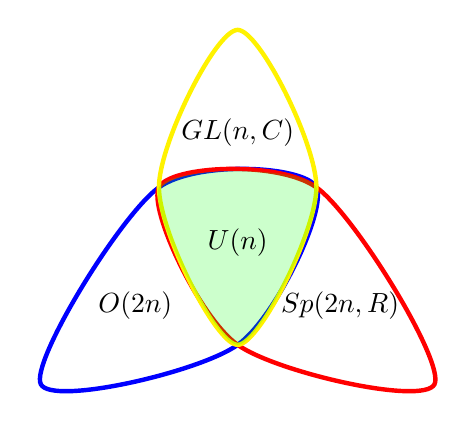
\begin{tikzpicture}
	\draw [blue, ultra thick] plot [smooth cycle] coordinates {(1,1) (0,-1) (-2.5,-1.5) (-1,1)};
	\draw [red, ultra thick] plot [smooth cycle] coordinates {(-1,1) (0,-1) (2.5,-1.5) (1,1)};
	\draw [yellow, ultra thick] plot [smooth cycle] coordinates {(0,3) (-1,1) (0,-1) (1,1)};
	
	\fill [green, opacity=.2] plot [smooth cycle] coordinates {(1,1) (0,-1) (-1,1)};
	
	\draw (-1.3,-.5) node [text = black] {$O(2n)$};
	\draw (1.3,-.5) node [text = black] {$Sp(2n, \mathbb{R})$};
	\draw (0,1.7) node [text = black] {$GL(n, \mathbb{C})$};
	\draw (0,.3) node [text = black] {$U(n)$};
%
%	\draw [gray!50, xshift=4cm]  (0,0) -- (1,1) -- (2,-2) -- (3,0);
%	\draw [cyan, xshift=4cm] plot [smooth, tension=2] coordinates { (0,0) (1,1) (2,-2) (3,0)};
\end{tikzpicture}


\end{document}
								\caption{%
									The intersection of two of the three groups of transformations $\GL(n, \mathbb{C})$, $\rmO(2n)$ and $\Sp(2n,\mathbb{R})$ is the same as the intersection of all the three. 
									It coincides with the group $\U(n)$ and gives an heuristic explanation of the fact that given two of the three structures, one can always build the third one.}
								\label{Uinters}
							\end{figure}
							%
						The $\omega$ in~\eqref{symeco} is non degenerate by construction (from~\eqref{hermetr}).
						On the other hand, given a pre-symplectic and an almost complex structures satisfying the compatibility condition,
							%
								\begin{equation}\label{hersym}
									\omega_{pq} I^{p}_{\phantom{p}m} I^{q}_{\phantom{q}n} = \omega_{mn}\, ,
								\end{equation}
							%
						it is always possible to define a metric
							%
								\begin{equation}\label{mesyco}
									g_{mn} = - \omega_{mp} I^{p}_{\phantom{p}n}\, ,
								\end{equation}
							%
						which is automatically Hermitian, from the~\eqref{I2mid}.
						Finally, as expected, a pre-symplectic structure and a metric always define an almost complex structure.
						The compatibility is given by the following condition,
							%
								\begin{equation}
									\omega^{T} g^{-1} \omega = g\, ,
								\end{equation}
							%
						while, one can explicitly build the almost complex structure via,
							%
								\begin{equation}
									I = - g^{-1} \omega\, .
								\end{equation}
							%
						%
					%
					\subsubsection{Identity structure}
						%
						Parallelisable manifolds are particularly relevant for supergravity compactifications.
						We define a parallelisable manifold in terms of vector fields and tangent spaces, follwoing~\cite{Nakahara}.
						
						Given a $d$-dimensional manifold $M$, a \emph{parallelisation} -- or \emph{absolute parallelism} -- of $M$ is a set $\{ v_1 ,\ldots, v_d\}$ of $d$ globally defined vector fields such that for all $p \in M$, the set $\{ v_1(p) ,\ldots, v_d(p)\} $ forms a basis for the tangent space in $p$, $T_p M$.
							
						If $M$ admits such a set, it is said to be \emph{parallelisable}.

						We can express the previous definition also saying that a manifold $M$ is parallelisable if admits a \emph{global frame}, since each basis vector $e_a$ is a globally defined smooth vector field.			
						From the point of view of $G$-structures, the existence of a parallelisation reduces the structure group to the identity element $\{e\}$.
						Because of this it is also said \emph{identity structure}, since transition functions on are actually identity maps, being the frame globally defined.
						This is equivalent to say that the parallelisation provides a global trivialisation of the tangent bundle $TM$.						
						Indeed, a parallelisation induces an isomorphism between tangent spaces in different points of the manifold.
						For example, aligning frames in each point, we can identify tangent spaces in that points. 
						%This assigns a connection with zero curvature to the manifold~\cite{paar}.
						
						An example of parallelisable manifolds are Lie groups.
						We can easily find a globally defined set of vector fields, forming a basis on $T_gG$ in each point $g \in G$. 
						These are the \emph{left(right)-invariant vector fields} $e_a$, which satisfy the Lie algebra
							%
							\begin{equation}
							\label{liealg}
								\left[e_a , e_b \right] = f_{ab}^{\phantom{ab}c}e_c\ ,
							\end{equation}
							%
						where $f_{ab}^{\phantom{ab}c}$ are constants called \emph{structure constants}.
						
						A further example is given by \emph{local group manifolds} \emph{i.e.} $ \mathcal{M} \cong G/\Gamma$, where $\Gamma$ is some discrete, freely-acting subgroup of the Lie group $G$.
						A possible parallelisation is given again by the left (right) invariant vector fields of $G$ if $\Gamma$ acts on the left (right). Moreover for any local group manifold, the parallelisation satisfies the~\eqref{liealg}.
						Technically, this happens because the condition $M = G / \Gamma$ implies that the left (right) invariant vector fields, which plays the role of generators of the Lie algebra $\mathfrak{g}$, must satisfy the commutation relations~\eqref{liealg}, with the structure constants that do not depend on the point on $M$.
						
						It is a well-known and remarkable result in algebraic topology -- due to Bott and Milnor et al. \cite{bott, Kervaire} -- that the only parallelisable spheres are $S^1,\ S^3,\ S^7$. This is related to the existence of the normed division algebras $\mathbb{C},\ \mathbb{H},\ \mathbb{O}$. 
						Another famous result is the non-existence of a parallelisation for a $2$-sphere. 
						This statement descends directly from the so-called \emph{hairy ball theorem}, a particular case of the \emph{Poincaré-Hopf theorem} that is considered very important since it provides a link between topological properties of manifolds and analytical ones \cite{adams, Hairy}.						
						
						Parallelisable manifolds (and their generalisation) will be very important to build maximally supersymmetric truncations of $10$- and $11$-dimensional supergravities, so we will analyse it in detail in the next chapters.
						%
				%
					%
					\subsubsection{\texorpdfstring{$\SU(n)$ structures}{SU(n) structures}}
						%
						In~\cref{almHermstruct}, we already mentioned that an almost complex structure and a compatible pre-symplectic structure reduce the structure group to $\U(d/2)$.
						In the case a globally defined $(n,0)$-form $\Omega$ (with $n = d/2$) exists associated to the almost complex structure, then we can define an orientation over the manifold and the structure group reduces further to $\SU(n)$.
						
						In terms of invariant tensors, an $\SU(n)$ structure is given by a globally defined, non-degenerate, simple $(n,0)$-form $\Omega$, a real non-degenerate two form $\omega$ and by an hermitian positive definite metric $g$.
						The forms $\omega$ and $\Omega$ satisfy the compatibility condition,
							%
								\begin{equation}\label{compatib1}
									\omega \wedge \Omega = 0\, .
								\end{equation}
							%
						The fundamental form $\Omega$ is usually normalised such that,
							%
								\begin{equation}\label{compatib2}
									\Omega \wedge \overline{\Omega} = (-1)^{[n/2]}\, \frac{(2i)^{n}}{n!} \omega^n = \mathrm{vol}_{d}\, .
								\end{equation}
							%
						The normalisation factors are chosen such that taking $n$ forms $\phi^i$ as a local basis of one-forms -- in which $\Omega$ takes the form~\eqref{Odec} -- the $\omega$ takes the canonical form,
							%
								\begin{equation}
									\omega = - \frac{i}{2} \sum_{i} \phi^i \wedge \bar{\phi}^i\, .
								\end{equation}
							%
						
						Let us assume that the manifold $M$ admits a spin structure. 
						We assume this having in mind to study supersymmetric background, which impose the internal manifold to be spin.
						Having a spin manifold means that the structure group $\SO(d)$ preserving metric and orientation can be lifted to $\mathrm{Spin}(d)$.
						Under these assumptions, we can equivalently define an $\SU(n)$ structure in terms of invariant spinors.
						
						We need some definitions.
						A spinor is said \emph{pure} if it is annihilated by half of the gamma matrices. Up to dimension $6$ this condition does not play any role, since any Weyl spinor is also pure. 
						However, in dimensions higher than $6$, this condition becomes relevant since it happens that exist spinors which are not pure.
						A concrete example is the case $d=7$, the only odd dimensional situation allowing for invariant spinors.
						The structure group reduces to $G_2$.
						
						A chiral pure spinor $\eta$, invariant under $\SU(n)$, reduces the structure group to $\SU(n)$.
						The inverse implication is also true.
						An $\SU(n)$-structure implies the existence of a globally defined, pure invariant spinor.
						This invariant spinor is related to the invariant forms we have seen above in terms of bilinears,
							%
								\begin{equation}\label{spinorSUn}
									\begin{split}
										\omega_{mn} &= i \eta^\dagger \gamma_{mn} \eta\, , \\
										\Omega_{mnp} &= \eta^T C \gamma_{mnp} \eta\, ,
									\end{split}
								\end{equation}
							%
						where $\gamma$ are the anti-symmetric products of gamma matrices of $\mathrm{Cliff}(d)$. 						%
						%%%
				\comment{It might be useful to add a section describing $\SU(2)$ and $\SU(3)$ structures.}
						%%%
				%
		\section{Holonomy and Torsion}
			%
				So far we discussed how the existence of certain invariant, globally defined objects is equivalent of a reduction of the structure group of the frame bundle.
				This is a topological notion. There are also differential conditions one can impose, which correspond to the notion of integrability of a structure.
				In the following of the thesis we will see how these differential conditions on the $G$-structures are related in string theory to the the condition that a given
				vacuum is supersymmetric. 
					\comment[w]{%
						I don't know whether to talk about integrability for distributions and Frobenius theorem.%
						}
					\comment{%
						We have seen, for instance in the case of an almost complex structure, that the (complexified) tangent bundle is split in sub-bundles corresponding to the eigenspaces of the structure.
						These sub-bundles are called \emph{distributions}.
						The integrability of the structures (when it is possible to associate them to a distribution) is related to the integrability of the corresponding distribution.
						For this reason we give the definition of the integrability for distributions first.%
						}%
					%
			%
			\subsection{Integrability of structures}
				%
					We will not give a rigorous definition of integrability.
					The curious reader can refer to many detailed references, a non-exhaustive list comprends~\cite{int1, int2, int3}.
					
					Heuristically we can say that an integrable structure (useful for our purposes) is a structure for which is possible to find a system of adapted coordinates on the manifold, such that the structure takes a particularly simple and fixed form.
					For our concerns, we will rephrase integrability in terms of intrinsic torsion.
					The structure is integrable if its compatible connection is torsion-free.
					We recover the notion of \emph{special holonomy} manifolds as the special case where all the torsions vanish.
					
					We now proceed with examples of integrability for the structures of the previous section in order to clarify the concepts.
				%
				\subsubsection{Complex structure}
					%
						Given an almost complex structure $I$, we say it is \emph{integrable} if and only if there exists a set of coordinates where it takes the form,
							%
								\begin{equation}
								\label{diagI}
									I =	\begin{pmatrix}
											i \id	&		0		\\
												0		&	i \id	\\
										\end{pmatrix} \, .
								\end{equation}
							%
						An integrable almost complex structure is called simply \emph{complex structure}.
						There are two equivalent definitions of integrability for an almost complex structure. 							%
								\begin{itemize}
									%
									\item[-]	The first one refers to the Nijenhuis tensor
									%
													\begin{equation}\label{nijten}
														N_I(v,w) := I \left[ I v, w \right] + I \left[ v, I w \right] - \left[ I v, I w \right] + \left[ v, w \right]\, ,
													\end{equation}
												%
									where $v, w$ is a pair of vector fields.
											One can prove $N_I$ is actually a tensor, since it depends only on the local value of $v, w$ at each point.
											One can show that $I$ is integrable if and only if
												%
													\begin{align*}
														& & N_I(v,w) = 0 & & \forall v, w\, .& &
													\end{align*}
												%
										%
									\item[-]	Alternatively, the complex structure $I$ is integrable if $TM^{(1,0)}$ part (and symmetrically the $TM^{(0,1)}$ part) are closed under the Lie bracket\footnote{
												Actually, this property of a distribution is called \emph{involutivity}. 
												A distribution is integrable if and only if it is involutive. 
												This is the content of the \emph{Frobenius theorem}.
												Because of the equivalence stated by the Frobenius theorem, often involutivity and integrability are concepts which are identified also in definitions.%
													}
													%
													\begin{align*}
														& &	P_{\mp} \left[ P_{\pm} v, P_{\pm} w \right] = 0	& &	\forall v,w \in TM \, .	& &
													\end{align*}
													%
												where $P_\pm$ are the projectors onto the $T^{(1,0)}$ and $T^{(0,1)}$. 
												That is, the Lie bracket of two (anti-)holomorphic vector fields must be (anti-)holomorphic.
											
												One can see that both the real and imaginary part of the relation above are proportional to $N_I$.
									%
								\end{itemize}
							%
						An almost complex manifold admitting a complex structure is said \emph{complex manifold}.
						We have seen that for almost complex manifolds possible to define complex coordinates in a single patch.
						For a complex manifold, the transition functions are holomorphic functions of the complex coordinates.
						Precisely, requiring holomorphic transition functions allows us to write the $I$ in the diagonal form~\eqref{diagI}.
					%
				\subsubsection{Symplectic structure}
					%
						The integrability for an almost symplectic structure is equivalent to the existence of a set of coordinates on $M$ such that
							%
								\begin{equation}
									\omega = \dd x_m \wedge \dd y^m\, ,
								\end{equation}
							%
						and such that the transition functions are symplectic with respect to the structure.
						Thanks to an important result in differential geometry, the Darboux theorem, we can translate integrability into a differential equation for the structure,
							%
								\begin{equation}
									\dd \omega = 0\, .
								\end{equation}
							%
						In other words, we simply demand the closure of the structure.
						
						With lack of fantasy, an integrable pre-symplectic structure is called \emph{symplectic structure} and a manifold endowed with it a \emph{symplectic manifold}.
						
					\paragraph{K\"ahler manifold} Following~\cite{KahlBook}, a \emph{K\"ahler manifold} is a complex manifold $(X, I, g)$ with an Hermitian metric $g$, whose associated symplectic structure $\omega$ is integrable.
					
					In other words, given the metric and the complex structure, the form constructed as in~\eqref{symeco} is closed,
						%
							\begin{equation}
								\dd \omega = 0\, .
							\end{equation}
						%
					When this happens, $\omega$ is called \emph{K\"ahler form}.
					%
				%
			%
			\subsection{Intrinsic torsion}
				%
					To any $G$-structure one can associate the notion of intrinsic torsion.
					This is because, as discussed in~\cref{gstruc} a $G$-structure can be seen as a principal bundle over the manifold $M$, with fibres given by the group $G$.
					On this bundle one can defines a connection, known as \emph{principal connection} and define its torsion.
					As argued in~\cite{joyce}, given a $G$-structure on $M$, a principal connection on the corresponding principal bundle always induces a connection $\nabla$ on the tangent bundle $TM$\footnote{%
						More precisely one can say that a general connection $D$ is compatible with a $G$-structure if and only if the corresponding connection on the principal frame bundle $F$, restricetd to the sub-bundle $P_G$ defining the $G$-structure, is still a connection on $P_G$~\cite{koba}.
						}.
					Such a connection is said to be \emph{compatible} with the structure and all the properties of the principal connection are inherited by the induced connection.
					For this reason we deal with connection on $TM$ and we are allowed to talk about torsion of the associated $G$-structure.
					
					We start the discussion about the intrinsic torsion by recalling the notion of compatibility of the connection on a manifold with a given structure.
					
					Let $(M,\Phi)$ be a manifold endowed with a $G$-structure defined by a tensor $\Phi$. A connection\footnote{%
						A connection $\nabla$ on a vector bundle $E$ is a map
							%
								\begin{align*}
									\nabla : \Gamma\left(E\right) \rightarrow \Gamma\left(E \otimes T^*M \right)\, ,
								\end{align*}
							%
						such that $\nabla(f v) = f \nabla(v) + v \otimes \dd f$, where $v$ is a section of $E$ and $f$ is a smooth function on $M$.%
						}	
					$\nabla$ on the tensor bundle is said to be \emph{compatible} with the structure if
						%
							\begin{equation}
								\nabla \Phi = 0 \, .
							\end{equation}
						%
					In general, given a structure the compatible connection is not unique.
					All the compatible connections differ by a tensor called \emph{torsion tensor},
						%
							\begin{equation}\label{torsmap}
								T_{\nabla} (v,w) = \left[\nabla_v w , \nabla_w v \right] - \left[v , w \right]\, ,
							\end{equation}
						%
					where $v$ and $w$ are generic sections of the tangent bundle and $[ \cdot, \cdot]$ the ordinary Lie bracket.
					
					In general given two different connections they will have a different torsion. 
					However, given a $G$-structure it is always possible to identify a part of the torsion which does not depend on the particular choice of the connection, but only on the $G$-structure.
					This part is called \emph{intrinsic torsion}.
					If the intrinsic torsion vanishes, then the associated $G$-structure is \emph{torsion-free}, \emph{i.e.} there exists at least one connection whose torsion tensor vanishes.
					The interesting fact we want to focus on is the identification of the integrability of the structure with its being torsion-free.
					
					Since we are interested in the application of these concepts in string theory compactifications, where we always deal with Riemannian manifolds, we are going to define intrinsic torsion in this case.
					For a rigorous definition of these notions for a generic manifold we refer again to~\cite{joyce}.
					%
				%
				\subsubsection{Metric compatible connection}
					%
				 A Riemannian manifold has $\rmO(d)$-structure.
						Then, in this case we consider a connection $\nabla$ compatible with the metric, 
							%
								\begin{equation}
									\nabla g = 0 \, .
								\end{equation}
							%
						We have a torsion free connection, if the torsion of the connection vanishes.
						The interesting fact about Riemannian compatible connections is that the torsion free metric compatible connection exists and is unique, the \emph{Levi-Civita connection}.
						This result is the content of the so-called \emph{fundamental theorem of Riemannian geometry}.
						This implies that any metric on $M$ defines an $\rmO(d)$-structure which is torsion free.
						For the following, let us further restrict our attention to orientable manifolds, \emph{i.e.} to $\SO(d)$-structures.
						
						Given a generic metric compatible connection, it can be written as,
							%
								\begin{equation}\label{contrs}
									\nabla = \nabla_{LC} + \kappa\, ,
								\end{equation}
							%
						where we denoted with $\nabla_{LC}$ the Levi-Civita connection and with $\kappa$ a tensor called the \emph{contorsion}.
						
						The contorsion $\kappa$ is the difference between a generic torsion full connection and the torsion free connection, both metric compatible.
						From the compatibility condition, we require,
							%
								\begin{equation}
									\kappa_{mnp} = - \kappa_{mpn}\, ,
								\end{equation}
							%
						where indices are lowered/raised by the metric.
						One can easily show that there is a one-to-one correspondence between the torsion and contorsion tensors,
							%
								\begin{align*}
									T_{mn}^{\phantom{mn}p} &= \kappa_{[mn]}^{\phantom{[mn]}p}\, , \\
									\kappa_{mnp} &= T_{mnp} + T_{pmn} + T_{npm} \, .
								\end{align*}
							%
						Hence, we will use the terms torsion and contorsion equivalently.
						
						A consequence of the correspondence between torsion and contorsion is that given a torsion $T$, we can build a connection which torsion $T$ and we are guaranteed that such a connection is actually unique.
						
						Let us now take the case where a further reduction of the structure group is possible. 
						That is, a globally-defined, invariant tensor under a group $G \subset \SO(d)$ exists.
						In general a $G$-structure compatible connection will satisfy
							%
								\begin{equation}
									\nabla g = \nabla \Phi = 0\, .
								\end{equation}
							%
						In general, there is no reason for the torsion of this connection to be zero.
						Thus, as we have seen above in~\eqref{contrs}, we write 
							%
								\begin{equation}
									\nabla \Phi = \nabla_{LC} \Phi + \kappa_0 \Phi = 0\, ,
								\end{equation}
							%
						where $\kappa_0$ is called \emph{intrinsic contorsion}\footnote{%
							Heuristically speaking, the intrinsic (con)torsion is the measure of the failure of the structure to be convariantly constant with respect the Levi-Civita connection.
							}.
						It is the bit of the contorsion acting non-trivially on the structure tensor.
						
						To be more explicit, let us consider the symmetry properties of the contorsion.
						$\kappa$ is an element of $T^*M \otimes \Lambda^2 T^*M$.
						Observe that the algebra of $\SO(d)$ -- here denoted as $\mathfrak{so}(d)$ -- is isomorphic to the (linear) space of two forms $\Lambda^2 T^*M$.
						Hence, the contorsion can be interpreted as a one form taking values on the $\mathfrak{so}(d)$ algebra,
							%
								\begin{equation}
									\kappa \in T^*M \otimes \mathfrak{so}(d)\, .
								\end{equation}
							%
						Let us denote by $\mathfrak{g}$ the sub algebra of $\mathfrak{so}(d)$ corresponding to the algebra of the group $G \subset \SO(d)$.
						We can split the map $\kappa$ in a piece taking values in $\mathfrak{g}$ and another part taking values in $\mathfrak{g}^{\perp}$, the orthogonal complement of $\mathfrak{g}$.
						Explicitly,
							%
								\begin{align}\label{decomk}
								&&	\kappa = \kappa_0 + \kappa_\mathfrak{g}\, , & & 	\begin{array}{l}
																				\kappa_0 			\in T^*M \otimes \mathfrak{g}^\perp \\[1mm]
																				\kappa_\mathfrak{g} \in T^*M \otimes \mathfrak{g}
																			\end{array}	&&
								\end{align}
							%
						Since $\Phi$ is $G$-invariant, the action on it of the generators of $G$ is trivial, \emph{i.e.} $g \cdot \Phi = 0$, $\forall g \in \mathfrak{g}$.
						So,
							%
								\begin{equation}
									\nabla \Phi = (\nabla_{LC} + \kappa_0 + \kappa_{\mathfrak{g}}) \Phi = (\nabla_{LC} + \kappa_0) \Phi = 0\, .
								\end{equation}
							%
						Thus, the difference between two $G$-compatible connections only lies in the $\kappa_{\mathfrak{g}}$ part of the contorsion.
						All the $G$-compatible connections share the same intrinsic contorsion $\kappa_0$, which is a property of the $G$-structure itself and not of the particular choice of the connection.
						
						The \emph{intrinsic torsion} is defined from the intrinsic contorsion 
							%
								\begin{equation}
									T^{0\phantom{mn}p}_{mn} = \kappa_{0[mn]}^{\phantom{0[mn]}p} \, .
								\end{equation}
							%
						The intrinsic torsion is a very important tool, since it provides a classification of $G$-structures.
						The idea is that it is possible to decompose $\kappa_0$ into irreducible representations of the group $G$.
						Then a $G$-structure will be specified in terms of the representations in `$\kappa_0$. 
						When $\kappa_0$ vanishes, for instance $\nabla_{LC}\Phi = 0$, the structure is torsion-free.
					%
				%
					%
				\subsubsection{Complex structure}
					%
						An almost complex structure reduces the structure group to $\GL(n, \mathbb{C})$.
						A compatible connection $\nabla$, as we have seen, is such that $\nabla I = 0$.
						In this case, we can show that the integrability of the structure is equivalent to to the vanishing of the intrinsic torsion of the $\GL(n, \mathbb{C})$-structure.
 						One can use $\nabla I = 0$ and the definition of torsion map~\eqref{torsmap} to show that, for any $v,w$, the Nijenhuis tensor~\eqref{nijten} can be written as
							%
								\begin{equation}
									N_{I} (v, w) = T_{\nabla} (v,w) - T_{\nabla} (Iv, Iw) + I T_{\nabla} (Iv,w) + I T_{\nabla} (v, Iw) \, .
								\end{equation}
							%
						Thus, being the Nijenhuis tensor proportional to the torsion tensor, if the latter vanishes so does the former, and the almost complex structure is integrable.
 						Since the equation above does not depend on the choice of a particular connection, the obstruction to the integrability of the almost complex structure only comes from the intrinsic torsion.
					%
				%
					%
				\subsubsection{Symplectic structure}
					%
						As already discussed, the pre-symplectic structure corresponds to a reduction of the structure group to $\Sp(d,\mathbb{R})$.
						We can find a torsion free compatible connection if and only if $\omega$ is integrable.
						Let us consider a compatible connection $\nabla$, $\nabla \omega = 0$.
						Then, one can show,
							%
								\begin{equation}
									\dd \omega (u, v, w) = \omega(T_\nabla (u,v), w) + \omega(T_\nabla (w,u), v) + \omega(T_\nabla (v,w), u)\, .
								\end{equation}
							%
						Hence the vanishing of the torsion tensor implies the closure (and so the integrability) of the structure.
						Also in this case, one can prove that the result does not depend on the particular choice of the connection, but on the intrinsic torsion of the $\Sp(d, \mathbb{R})$-structure only.
					%
				%	
			%
			\subsection{Special Holonomy}
				%
					We want now to analyse another differential property of a manifold: the \emph{holonomy} of a connection.
					This concept will be deeply related to supersymmetry in string compactifications.

					
					Let us consider a manifold $M$ and a differentiable\footnote{%
						In the rest of this thesis, unless specifically indicated, we will not distinguish between continuity and differentiability. In other words, a $\mathcal{C}^0$ function will always be also $\mathcal{C}^\infty$ and an homeomorphism will always be also a diffeomorphism.%
						}
					curve $\gamma$ on it, \emph{i.e.} $\gamma : I \rightarrow M$, where $I$ is a real open interval.
					Then, let $E$ be a vector bundle over its base manifold $M$ and $\nabla$ a connection on $E$. 
					The connection $\nabla$ provides a way of moving elements of the fibres along a curve. 
					In particular, it defines an isomorphisms between the fibres at different points along the curve, the so-called \emph{parallel transport} map,
						%
							\begin{align}
								& & & & P_\gamma : E_{\gamma(s)} \rightarrow E_{\gamma(t)} & & \forall t,s \in I\, .
							\end{align}
						%
					
					Let us now consider a \emph{loop}, \emph{i.e.} a closed curve, based at a point $x \in M$, then the parallel transport is an automorphism of the vector bundle at the point $x$,
						%
							\begin{equation}
								P_\gamma : E_{x} \rightarrow E_{x}\, .
							\end{equation}
						%
					As said, the map $P_\gamma$ is an automorphism, so both linear and invertible.
					It is an element of $\GL(E_x) \cong \GL(k, \mathbb{R})$, where $k$ is the dimension of the fibres.
					The set of all the possible parallel transports, for the all possible loops based at $x$ defines the \emph{holonomy group} of the connection $\nabla$ based at $x$,
						%
							\begin{equation*}
								\mathrm{Hol}_x (\nabla) := \left\{ P_\gamma \mid \gamma \text{ based at } x \right\}\, .
							\end{equation*}
						%
					In the case of a simply connected manifold $M$, the holonomy group depends on the base point only up to conjugation by an element of $\GL(k,\mathbb{R})$.
					More explicitly, if $\psi$ is a path connecting $x$ to $y$ in $M$, then
						%
							\begin{equation*}
								\mathrm{Hol}_x (\nabla) = P_\psi^{\vphantom{-1}}\ \mathrm{Hol}_y (\nabla)\ P_\psi^{-1}\, .
							\end{equation*}
						%
					Hence, given this relation one often (and we will follow this use) drops the reference to the base point, understanding that the definition holds up to group element conjugation.
					
					An important fact about holonomy is that given a a connection on a vector bundle, there is a relation between the action of the holonomy algebra $\mathfrak{hol}(\nabla)$ and the curvature of the connection (for detail on can read~\cite{holon2}).
					Recall that the curvature of a connection $\nabla$ is a two-form $R$ taking values in the Lie algebra\footnote{%
						One can write a connection as the differential operator,
							%
								\begin{equation*}
									\nabla = \dd + A \, ,
								\end{equation*}
							%
						where A is a one-form with values in the Lie algebra of the structure group of M, also called (often misleading) \emph{connection}.
						On a coordinate basis, the connection has the familiar form in physics literature: $\nabla = \dd x^m \otimes \nabla_m$, where and $\nabla_m$ is usually known as covariant derivative.
						
						The \emph{curvature} of the connection is defined as the two-form
							%
							\begin{equation*}
								R := \dd A + \frac{1}{2} \left[A , A\right]\, .
							\end{equation*}
						}
					of the structure group.
					
					Consider now a tensor bundle over a manifold $M$ and suppose that this admits a covariantly constant tensor,
						%
							\begin{equation*}
								\nabla \Phi = 0\, .
							\end{equation*}
						%
					Then this tensor is invariant under parallel transport, and so also under the holonomy group.
					As a consequence the holonomy group cannot be the full $\GL(d, \mathbb{R})$, but it must be a subgroup, precisely the one leaving $\Phi$ invariant.
					The opposite statement holds as well, every time we have a reduced holonomy group, there exists an invariant object.
					In this case we say the manifold has a \emph{reduced holonomy}.
					
					Let us consider a connection with reduced holonomy. 
					We know we can always write it as $\nabla = \nabla_{LC} + \kappa_0$.
					This implies one can always find a $G$-structure such that the holonomy group corresponds to $G$, \emph{i.e.} $\mathrm{Hol}(\nabla) = G$.
					If the connection is Levi-Civita, then the corresponding $G$-structure is torsion-free.
						%
							\begin{table}[h!]
							\centering
								\begin{tabular}{c | c | c | c}
%									\toprule
									Holonomy					&			dim($M$)							&	invariant tensors		&	Manifold				\\
									\midrule
									$\SO(d)$					& 			$d$								&	$g, \mathrm{vol}_g$		&	(Riemannian) Orientable	\\[1.2mm]
									$\U(n) $	 				&			$d = 2n$							&	$g, \omega$			&	K\"ahler				\\[1.2mm]
									$\SU(n)$		 			&			$d = 2n$							&	$\omega, \Omega$		&	Calabi-Yau			\\[1.2mm]
									$\Sp(n)$		 			&			$d = 4n$							&						&	Hyperk\"ahler			\\[1.2mm]
									$\Sp(n) \Sp(1)$				&			$d = 4n$							&						&	Quaternionic K\"ahler	\\[1.2mm]
									$\mathrm{G}_2$		 	&			$d = 7$							&		$\phi_3$			&	$\mathrm{G}_2$		\\[1.2mm]
									$\mathrm{Spin}_7$		 	&			$d = 8$							&		$\Omega_4$		&	$\mathrm{Spin}_7$		\\
									\bottomrule
								\end{tabular}
								\caption{Various reduced holonomies.}
								\label{tabhol}
							\end{table}
						%			
				%		
			%
			\section{Examples: Calabi-Yau and Sasaki-Einstein}
			\label{CYSE}
				%
				Here we want to discuss two very important examples of manifolds with reduced holonomy: \emph{Calabi-Yau} and \emph{Sasaki-Einstein} manifolds.
				The former are even-dimensional manifolds, while the latter are odd-dimensional.
				The aim of this section is not to be complete, but to give the needed concepts for what follows in the thesis.
				A more complete source of informations (and of references) is~\cite{CalabiYauReview} for Calabi-Yau manifolds, and~\cite{SparksSE} for Sasaki-Einstein ones.
				
				We already restricted our attention to spin manifolds, since we are interested in supergravity compactifications.
				Here we want to justify this choice, saying that this is not too restrictive, since following~\cite[prop. 3.6.2]{joyce}, given a $d$-dimensional manifold $M$, with $d \geq 3$, admitting $G$-structure with $G$ simply-connected subgroup of $\SO(d)$, then $M$ is spin.
				
				For the sake of concreteness, let us restrict to the case of a six-dimensional manifold. 
				These manifolds are of particular interest since they appear in compactifications of ten-dimensional type II string theory down to four dimensions.
				The structure group $\GL(6)$ is reduced to $\SO(6) \simeq \SU(4)$ by the presence of a metric and an orientation defined by the latter.
				A globally defined spinor reduces further the structure group. The irreducible spinor representation is the $\mathbf{4}$. 
				Given a nowhere vanishing spinor $\eta$ we can always go to a frame where it takes the form $\left(0,0,0,s\right)$. 
				The $\SU(4)$ transformations leaving this invariant are precisely $\SU(3)$.
				Looking at $\SU(4)$ decomposition under $\SU(3)$, one can see that in the fundamental $\mathbf{4}$ there is a singlet under $\SU(3)$.
					%
						\begin{equation*}
							\begin{array}{rccr}
								\SU(4) 			&	\rightarrow	&	\SU(3)					&					\\
								\mathbf{4}			&	\rightarrow	&	\mathbf{3} + \mathbf{1}		&	\eta_+			\\
								\mathbf{\bar{4}}		&	\rightarrow	&	\mathbf{\bar{3}} + \mathbf{1}	&	\eta_+^*					
							\end{array}
						\end{equation*}
					%
				We have chosen our $6$-dimensional gamma matrices such that $\eta_+^*$ has opposite chirality.
				
				Hence, a globally defined spinor defines an $\SU(3)$-structure.
				This is also given by globally defined, nowhere-vanishing and invariant $2$-form and $3$-form satisfying compatibility conditions~\eqref{compatib1} and~\eqref{compatib2}, that is
					%
						\begin{align*}
							\omega \wedge \Omega &= 0\, , \\
							\Omega \wedge \bar{\Omega} &= \frac{4}{3} \omega^3\, .
						\end{align*}
					%
				
%				The structure group $\SU(3)$ is a subgroup of $\SO(6)$.
%				Thus, any form on $M$ (from $1$ to $6$) transforms in an irreducible representation of $\SO(6)$.
%				The idea is to decompose the all possible forms under $\SU(3)$ and look for the singlets of the structure, these are quantities that can be written in terms of the invariant tensors.
%					%
%						\begin{equation*}
%							\begin{array}{lcrcc}
%										&		\SO(6)		&	\rightarrow	&	\SU(3)										&								\\
%								\alpha_1	&	\mathbf{6}			&	\rightarrow	&	\mathbf{3} + \mathbf{\bar{3}}						&								\\
%								\alpha_2	&	\mathbf{15}		&	\rightarrow	&	\mathbf{8} + \mathbf{3} + \mathbf{\bar{3}} +\mathbf{1}	&	\omega						\\
%								\alpha_3	&	\mathbf{10}_c		&	\rightarrow	&	\mathbf{6} + \mathbf{3} + \mathbf{1}					&	\Omega						\\
%								\alpha_4	&	\mathbf{15}		&	\rightarrow	&	\mathbf{8} + \mathbf{3} + \mathbf{\bar{3}} +\mathbf{1}	&	\omega \wedge \omega 			\\
%								\alpha_5	&	\mathbf{6}			&	\rightarrow	&	\mathbf{3} + \mathbf{\bar{3}}						&	\omega \wedge \Omega = 0		\\
%								\alpha_6	&	\mathbf{1}			&	\rightarrow	&	\mathbf{1} 									&	\omega^3 \propto \Omega \wedge \bar{\Omega}
%							\end{array}
%						\end{equation*}
					%
				
				Consider now a connection $\nabla$ compatible with the $\SU(3)$-structure,
					%
						\begin{equation}\label{covdereta}
							\nabla \eta_+ = \nabla_{LC} \eta_+ + \kappa \cdot \eta_+ = 0\, .
						\end{equation}
					%
				where the contorsion $\kappa$ acts on spinors as,
					%
						\begin{equation}
							(\kappa \cdot \eta_+)_{m}^{\alpha} = \frac{1}{4} \kappa_{mnp} \gamma^{np, \alpha}_{\phantom{np,\alpha}\beta} \eta_{+}^\beta \, .
						\end{equation}
					%
				Again, we can see the (con)torsion as the obstruction to $\eta_+$ or ($\omega$ and $\Omega$) to be covariantly constant with respect to the Levi-Civita connection.
				
				The fact that $\eta_+$ is covariantly constant with respect to the connection $\nabla$ means that $\nabla$ has holonomy $\SU(3)$.
			For $d=6$, the decomposition~\eqref{decomk} takes the following form,
					%
						\begin{align}
							&&	\kappa = \kappa_0 + \kappa_{\mathfrak{su}(3)}\, , & & 	\begin{array}{l}
																				\kappa_0 			\in T^*M \otimes \mathfrak{su}(3)^\perp \\[1mm]
																				\kappa_{\mathfrak{su}(3)} \in T^*M \otimes \mathfrak{su}(3)
																			\end{array}	&&
						\end{align}
					%
				where we used the fact $\mathfrak{so}(6) \cong \mathfrak{su}(4) \cong \mathfrak{su}(3) \oplus \mathfrak{su}(3)^\perp$.
				We can now apply the contorsion decomposition to the expression for $\nabla \eta_+$, the~\eqref{covdereta}.
				Recall that since $\eta_+$ is an $\SU(3)$ singlet, one has
					%
						\begin{equation}
							\kappa_{\mathfrak{su}(3)} \cdot \eta_+ = 0\, .
						\end{equation}
					%
				Hence, one is left with
					%
						\begin{equation}\label{conteta}
							\nabla_{LC} \eta_+ = \kappa_0 \cdot \eta_+\, .
						\end{equation}
					%
				%Because of the isomorphic map between torsion and contorsion, we can now make use of the torsion tensor for the following discussion.

				The intrinsic contorsion and, hence, the intrinsic torsion $T^0$ can be decomposed into irreducible representations of $\SU(3)$					%
						\begin{equation*}
							\begin{array}{rrl}
								T^0 \in T^*M \otimes \mathfrak{su}(3)^{\perp}	& \rightarrow &	\left(\mathbf{3} \oplus \mathbf{\bar{3}}\right) \otimes \left(\mathbf{1} \oplus \mathbf{3} \oplus \mathbf{\bar{3}}\right)	\\[1.5mm]
																	& \rightarrow &	\underbrace{\left(\mathbf{1} \oplus \mathbf{1} \right)}_{W_1} \oplus \underbrace{\left(\mathbf{8} \oplus \mathbf{8} \right)}_{W_2} \oplus \underbrace{\left(\mathbf{6} \oplus \mathbf{6} \right)}_{W_3} \oplus \underbrace{\left(\mathbf{3} \oplus \mathbf{\bar{3}} \right)}_{W_4} \oplus \underbrace{\left(\mathbf{3} \oplus \mathbf{\bar{3}} \right)^\prime}_{W_5} \, .
							\end{array}
						\end{equation*}
					%
				The $W_i$ are called \emph{torsion classes}~\cite{TorsClass1, TorsClass2}. These can be seen as equivalence classes, meaning that all the structures sharing the same intrinsic torsion (or being in the same irrep of $SU(3)$) are equivalent. The representatives of the torsion classes are differential forms of different ranks, see~\cref{tabW}.
					%
						\begin{table}[h!]
						\centering
							\begin{tabular}{| c | l |}
								\toprule
								Form						&			rank								\\
								\hline
								$W_1$					& 			complex scalar						\\	
								$W_2 $	 				&			complex primitive $(1,1)$-form			\\	
								$W_3$		 			&			real primitive $(2,1) + (1,2)$-form		\\	
								$W_4$		 			&			real one-form						\\	
								$W_5$					&			complex $(1,0)$-form				\\
								\bottomrule
							\end{tabular}
							\caption{Torsion classes as differential forms.}
							\label{tabW}
						\end{table}
					%
				
				Recall that a form $\alpha$ is said \emph{primitive} if it has a zero contraction with $\omega$, \emph{i.e.} $\omega\lrcorner \alpha = 0$~\cite{joyce}.
				
				The torsions classes can be used also to express the integrability of the structure as differential conditions on the forms $\omega$ and $\Omega$				%
						\begin{subequations}
						\label{diffstruct}
							\begin{align}
								\dd \omega 	&= \frac{3}{2} \IIm \left( \overline{W}_1 \Omega \right) + W_4 \wedge \omega + W_3 \, , \\
								\dd \Omega	&= W_1 \wedge \omega \wedge \omega + W_2 \wedge \omega + \overline{W}_5 \wedge \Omega \, ,
							\end{align}
						\end{subequations}
					%
				
				These formulae allow to classify the manifolds with $\SU(3)$ structures through the torsion classes.
				We collect some example in~\cref{tabTorsCl},
					%
						\begin{table}[h!]
						\centering
							\begin{tabular}{l | l}
								Torsion Classes						&			Name							\\
								\hline
																	&											\\[-.3mm]
								$W_1 = W_2 = 0$						& 			Complex manifold					\\[1.5mm]	
								$W_1 = W_2 = W_4 = 0$					&			Symplectic manifold					\\[1.5mm]	
								$W_2 = W_3 = W_4 = W_5 = 0$ 			&			Nearly K\"ahler	manifold				\\[1.5mm]
								$W_1 = W_2 = W_3 = W_4 = 0$			&			K\"ahler manifold					\\[1.5mm]	
								$\IIm W_1 = \IIm W_2 = W_4 = W_5 = 0$		&			Half-flat manifold					\\[1.5mm]
								$W_1 = \IIm W_2 = W_3 = W_4 = W_5 = 0$ 	&			Nearly Calabi-Yau three-fold			\\[1.5mm]	
								$W_1 = W_2 = W_3 = W_4 = W_5 = 0$ 		&			Calabi-Yau three-fold					
							\end{tabular}
							\caption{Six-dimensional manifolds with $\SU(3)$ structure, classified by torsion classes.}
							\label{tabTorsCl}
						\end{table}
					%
				%
				\subsubsection{Calabi-Yau manifolds}
					%
					We saw that a $d$-dimensional K\"ahler manifold can be defined as a Riemannian manifold of even dimension $d=2n$, whose 
					holonomy group is contained in $\U(n)$.
					
					In the same way we can define Calabi-Yau manifolds as K\"ahler manifolds whose holonomy group is contained in $\SU(n)$. More precisely			
									given a compact K\"ahler manifold $M$ of complex dimension $n$, with complex structure $I$, Hermitian K\"ahler metric $g$ and associated K\"ahler form $\omega$, then $(M, I, g, \omega)$ is a \emph{Calabi-Yau $n$-fold} if and only if $g$ has $\SU(n)$ holonomy.
						
						%
%							\begin{definition}[Calabi-Yau $n$-fold]
%								\label{CYdef}
									Given a compact K\"ahler manifold $M$ of complex dimension $n$, with complex structure $I$, Hermitian K\"ahler metric $g$ and associated K\"ahler form $\omega$, then $(M, I, g, \omega)$ is a \emph{Calabi-Yau $n$-fold} if and only if $g$ has $\SU(n)$ holonomy.
%							\end{definition}
					

We can also define a Calabi-Yau manifold in terms of the structures $\omega$ and $\Omega$: a Calabi-Yau structure on an $2n$-dimensional manifold $M$ is the set $(M, \omega, \Omega)$, where $\omega$ and $\Omega$ are respectively an integrable K\"ahler two-form and a complex simple $n$-form defining an integrable complex structure
							\begin{align*}
								\dd \omega 	&= 0 \, , \\
								\dd \Omega	&= 0 \, ,
							\end{align*}
that are also compatible, \emph{i.e.} $\omega \wedge \Omega = 0$, and whose metric, defined as in~\eqref{mesyco}, is Ricci-flat, \emph{i.e.} $R = 0$.

	%
One can also show that this is equivalent to say that a Calai-Yau $n$-fold is a complex manifold, with a compatible (integrable) symplectic structure where in addition the metric associated as in~\eqref{mesyco} is Hermitian and Ricci-flat, \emph{i.e.} $R_g = 0$~\cite{joyce, KahlBook}\footnote{%
						The equivalence of these definitions is actually a consequence of the famous \emph{Calabi conjecture}~\cite{CalabiMetr}, proven by Yau~\cite{YauCalabi}, and so these manifolds were named after them.}.
						
					The standard example of trivial Calabi-Yau manifolds are the even-dimensional tori, equipped with the usual complex structure and metric.
					These are also the only Calabi-Yau compact manifolds for which an explicit Ricci-flat metric is known.
					For all the others, the Calabi theorem guarantees the existence of such a metric, but there is no explicit known construction yet.

						%
							

						%
					%
				%
				\subsubsection{Sasaki-Einstein manifolds}
					%
					Sasaki-Einstein manifolds are odd-dimensional manifolds, that are both Sasakian and Einstein.
					Then, let us start with thes definition of a Sasakian manifold~\cite{SparksSE}.

					A Riemannian manifold $(S,g)$ is \emph{Sasakian} if and only if its metric cone
										%
											\begin{equation*}
												C(S) := \mathbb{R}^+ \times S \, ,
											\end{equation*}
										%
					equipped with the metric $\overline{g} = \dd t^2 + t^2 g$, is a K\"ahler manifold.
					
					As first consequence of this definition, we can see that $S$ has to be odd dimensional, \emph{i.e.} $d=2n-1$, where $n$ is the complex dimension of the K\"ahler cone.
					
					An Einstein manifold, on the other hand, is a manifold equipped with an Einstein metric $g$, \emph{i.e.} a metric whose Ricci curvature is proportional to the metric itself,
						%
							\begin{equation*}
								R_g = \lambda g \, , 
							\end{equation*}
						%
					for some real constant $\lambda$.
					For a Sasakian manifold, it turns out that $\lambda = 2(n-1)$. Moreover, one can show that a Sasakian manifold is Einstein if and only if its cone is K\"ahler-Einstein and Ricci flat, namely a Calabi-Yau~\cite{SparksSE}.
					Hence, for a Sasaki-Einstein manifold, the restricted holonomy group\footnote{%
						The restricted holonomy group is the component of the group connected to the identity element.%
						}
					of its cone is $\mathrm{Hol}^0 (\overline{g}) \subset \SU(n)$.
					
					The standard example is provided by the odd-dimensional spheres $S^{2n-1}$, equipped with the standard Einstein metric.
					In this case the K\"ahler cone is simply the space $\mathbb{C}^n / {0}$, with the standard Euclidean metric.
					
					A Sasakian manifolds inherits some properties from the K\"ahler structure of its cone.
					One of the most important one for our concerns is the \emph{contact structure}~\cite{contact1}, represented by a nowhere-vanishing vector field $\xi$, known as \emph{Reeb vector field}.
					Using the coordinate $t$ to parametrise the $\mathbb{R}^+$ direction on the cone, we can write
						%
							\begin{equation}\label{Reeb1}
								\xi = I\left[ t \partial_t \right]\, ,
							\end{equation}
						%
					where $I$ is the complex structure on the cone.
					We will see how the Reeb vector will play an important role in compactifications of type IIB supergravities~\cite{DavideSas1, DavideTriSas} and further in the definitions of generalised structures~\cite{AshmoreESE}.
					
					As we have seen in the last section, on Calabi-Yau manifolds the group structure defines a covariantly constant spinor.
					On a Sasaki-Einstein, we have \emph{Killing spinors}, \emph{i.e.} a spinor $\psi$ such that
						%
							\begin{equation}
								\nabla \psi = \pm \frac{1}{2} \gamma \psi \, . 
							\end{equation}
						%
%					namely an eigenstate of the covariant derivative.
%					They can be seen as supersymmetry generators.
%					 
			A generic Sasaki-Einstein manifold supports two Killing spinors.

%, then, in the case of Freund-Rubin~\cite{FreundRubin} compactification on the $\mathrm{AdS}_4$-solution, we have an $\mathcal{N}=2$ supersymmetry~\cite{duffKK}.
					
					In addition, we can characterise a Sasaki-Einstein manifold equivalently by differential forms with compatibility relations among them.
					Explicitly, a \emph{Sasaki-Einstein structure} on a manifold $M$ is the set $(M, \xi, \sigma, \omega, \Omega)$, where $\xi$ is the Reeb vector of~\eqref{Reeb1}, $\sigma$ the dual one-form defined by $\sigma\left[X \right] = g(\xi, X)$\footnote{%
						Note that the metric $g$ is defined by the two compatible structures $\omega$ and $\Omega$ as in~\eqref{mesyco}. More precisely, the complex and symplectic structure on the K\"ahler cone define a metric $\overline{g}$, whose restriction gives $g$.%
						},
					$\omega$ is a real two-form and $\Omega$ a complex simple $n$-form.
					They have to satisfy the following relations,
						%
							\begin{equation}
								\begin{array}{c c c}
									\omega \wedge \Omega = 0 \, ,	&	\phantom{\dd}	&\iota_\xi \omega = \iota_\xi \Omega = 0 \, , \\[2mm]
									\dd \sigma = 2 \omega \, ,		&	\phantom{\dd}	&\dd \Omega = (n+1) i \sigma \wedge \Omega \, .
								\end{array}
							\end{equation}
						%
					Note that given a Sasaki-Einstein manifold, its metric can always be re-written as,
						%
							\begin{equation}
								\dd s^2 = \sigma \otimes \sigma + \dd s^2_{KE} \, ,
							\end{equation}
						%
					where $\dd s^2_{KE}$ is the metric on a generic K\"ahler-Einstein base.
					From this, we can say that the Reeb vector defines a \emph{foliation}, \emph{i.e.} it splits the tangent bundle into integral sub-bundles, whose set of leaves is a K\"ahler-Einstein space.
					Such a foliation is called (not surprisingly) \emph{Reeb foliation}.
					
					
Sasaki-Einstein manifolds are very common in string compactifications.
%and as for the Calabi-Yau spaces in $10$-dimensional supergravities, Sasaki-Einstein manifolds provide the internal space for the $11$-dimensional supergravity to $\mathrm{AdS}_4$~\cite{duffKK}. 
Recently, making use of their geometry has allowed to achieve several interesting results both in flux compactification and in a wider area of research in string theory~\cite{DavideTriSas, DavideSas1, SE1, SE2, SE3, SE4, SE5}.
					
					\paragraph{Tri-Sasakian Manifolds} 
					There is a sub-class of the Sasaki-Einstein manifolds, the so-called \emph{Tri-Sasakian manifolds} which is interesting not only because it has applications in flux compactifications~\cite{DavideTriSas}, but also simply to show how reduced holonomy gives rise to structures with different properties~\cite{TriSasakiReview}.
					
					In order to define this class of manifolds, we have to give the definition of \emph{Hyperk\"ahler manifold}.
					An hyperk\"ahler manifold is a Riemannian manifold $(M,g)$ of dimension $4k$ whose holonomy group $\mathrm{Hol}(g)$ is contained in the symplectic group $\Sp(k)$.
					Note that all hyperk\"ahler manifolds are also Calabi-Yau (the metric $g$ is Ricci-flat), since $\Sp(k) \subset \SU(2k)$.
					
					We are interested in the structures defined on this kind of manifolds.
					An hyperk\"ahler manifold has a set of three complex structures $\{I, J, K\}$ with respect to which the metric is K\"ahler.
					The three complex structures respect the Hamilton algebra of quaternions~\cite{EncyclMath},
						%
							\begin{equation}
								I^2 = J^2 = K^2 = - \id \, ,
							\end{equation}
						%
					and they also have the property that any linear combination with real coefficients $\alpha I + \beta J + \gamma K$, and $\alpha^2 + \beta^2 + \gamma^2 = 1$ is a complex structure on $M$.
					Because of these one can say that the tangent space at any point is a quaternionic vector space.
					
					A \emph{tri-Sasakian manifold} is a Sasaki-Einstein manifold whose cone is hyperk\"ahler.
					This definition constrains the dimension of a tri-Sasakian manifold to be $4n+3$, with $n \geq 1$.
					We can also give an equivalent characterisation in terms of tensors defining structures.
					
					A tri-Sasakian manifold has three mutual orthogonal Killing vectors $\xi_i$, such that each of them is a Reeb vector, and all together they generate an $\SU(2)$ algebra,
						%
							\begin{equation}
								\left[\xi_i , \xi_j \right] = 2 \epsilon_{ij}^{\phantom{ij}k} \xi_k \, .
							\end{equation}
						%
					They also have their associated dual contact forms, \emph{i.e.} $\sigma^i$ such that $\sigma^i (\xi_j) = \delta^i_j$.
					Each $\sigma^i$ satisfies the differential relation,
						%
							\begin{equation}
								\dd \sigma^i = 2 J^i - \epsilon_{\phantom{i}jk}^i \sigma^j \wedge \sigma^k \, ,
							\end{equation}
						%
					where $\iota_{\xi_i}J^{j} = 0$.
					Taking the exterior derivative of the relation above one gets
						%
							\begin{equation}
								\dd J^i = 2 \epsilon^{i}_{\phantom{i}jk} J^j \wedge J^k \, .
							\end{equation}
						%
					
					As one may expect, the three Reeb vectors define what is known under the name of \emph{tri-Sasakian foliation}, whose space of leaves is a quaternionic K\"ahler space (whose holonomy group is contained in $\Sp(n)\Sp(1)$) $B_{QK}$, and the metric on the tri-Sasaki can be written as,
						%
							\begin{equation}
								\dd s^2 = \dd s^2_{B_{QK}} + \sigma^i \otimes \sigma ^i \, .
							\end{equation}
						%
					To conclude this discussion, we want to make the following remark.
					For any linear combination $\alpha^i \xi_i$ with $\alpha^i \alpha^i =1$, we can define a Sasaki-Einstein structure through,
						%
							\begin{align*}
								\sigma &= \alpha_i \sigma^i \, , \\
								\omega &= \alpha_i \left(J^i - \frac{1}{2} \epsilon^i_{\phantom{i}jk} \sigma^j \wedge \sigma^k \right) \, , \\
								\Omega &= \left(\beta_j \sigma^j - i \gamma_j \sigma^j \right) \wedge \left(\beta_k J^k - i \gamma_k J^k \right)\, ,
							\end{align*}
						%
					where $\beta_i$ and $\gamma_i$ are sets of coefficients such that $\beta^i \xi_i$ and $\gamma^i \xi_i$ are mutually orthogonal.
					The coefficients (up to the orthogonality condition) can be chosen arbitrarily, since the various choices gives the same Sasaki-Einstein structures up to the phase of $\Omega$.
%					This freedom in the choice of the phase reflects in the fact that studying a compactification on a Sasaki-Einstein structure, the authors of~\cite{Gauntlett:2009zw} found an extra $\U(1)$ symmetry.
					%
				%
			%
		%
\end{document}